\documentclass[notes]{beamer}

\usetheme{Darmstadt}
\usepackage{lmodern}% http://ctan.org/pkg/lm
\usepackage{amsthm,amstext,amsfonts,bm,amssymb}

\mode<presentation>
%\useoutertheme{smoothbars}
\useinnertheme[shadow=true]{rounded}
\usecolortheme{whale}
\useoutertheme{split}
\usefonttheme[onlysmall]{structurebold}
\usefonttheme{professionalfonts}
\usepackage{amssymb}
\usepackage{verbatim}
%\setbeamertemplate{footline}[frame number]
\mode
<all>

\usepackage{algorithmic}
\usepackage{algorithm}
\renewcommand{\algorithmicrequire}{\textbf{Input:}}
\renewcommand{\algorithmicensure}{\textbf{Output:}}
\newcommand{\algorithmiclocal}{\textbf{Local Variables: }}
\newcommand{\LOCAL}{\item[\algorithmiclocal]}
\newcommand{\algorithmicsend}{\textbf{send }}
\newcommand{\algorithmicreceive}{\textbf{receive }}
\newcommand{\SEND}{\algorithmicsend}
\newcommand{\RECEIVE}{\algorithmicreceive}
\newcommand{\true}{\textbf{true}}
\newcommand{\false}{\textbf{false}}

\newcommand{\red}{\textcolor{red}{red }}
\newcommand{\blue}{\textcolor{blue}{blue }}
%\newcommand{\<--}{$\longleftarrow$}
%\newcommand{\<-}{$\leftarrow$}
%\newcommand{\-->}{$\longrightarrow$}
%\newcommand{\->}{$\rightarrow$}

% % % % % margin notes % % % % % %

%\usepackage{cooltooltips}
%\def\cool{\texttt{cool}}

%\usepackage[margin=1cm]{caption}
\usepackage[colorinlistoftodos,prependcaption
,textsize=tiny
]{todonotes}

%\reversemarginpar
%\newcommand\todoil[1]{\todo[inline]{ #1}}
\newcommand\todoil[1]{ {\color{red}\textit{#1}}\todo[disable]{#1}}
% % % % % % % end % % % % % % % %

%%%%%%%% Packages for drawing diagrams %%%%%%%%%%%%%%%
\usepackage{tikz,ifthen}
\usetikzlibrary{arrows,automata,positioning }
\tikzstyle{block}=[rectangle, draw, thin, inner sep=3pt, text centered, 
%drop shadow, 
fill=orange!20!yellow!20] 
\tikzstyle{pre}=[<-,shorten <=1pt,>=stealth']
\tikzstyle{post}=[->,shorten >=1pt,>=stealth'] 
\tikzstyle{bi}=[<->,shorten >=1pt,shorten <=1pt,>=stealth'] 
\tikzstyle{every initial by arrow}=[initial text={},initial distance=1em,post]
%\tikzstyle{every state}=[minimum size=0.4cm,drop shadow,fill=orange!20!yellow!20]
\tikzstyle{transition}= [post,shorten >=1pt,node distance=2cm, inner sep=2pt,bend angle=20]
\tikzstyle{box}=[rectangle,draw=black, thick, inner sep=3pt, text centered]

%Hodai part
%\usepackage{tikz}
\usetikzlibrary{shapes.geometric, arrows, automata, positioning}
\tikzstyle{recNode} = [rectangle, minimum width=2cm, minimum height=1cm, text centered, rounded corners=0.1cm, draw=black]
\tikzstyle{recNodeB} = [recNode, draw=blue, fill=blue!10,text=blue!20!black]
\tikzstyle{recNodeG} = [recNode, draw=red, fill=red!10,text=red!10!black]
\tikzstyle{eNode} = [minimum height=1cm, text centered,text=blue!20!black]

\tikzstyle{arrow} = [thick,->,>=stealth,draw=black]
\tikzstyle{arrowB} = [thick,->,>=stealth,draw=blue]
\tikzstyle{arrowG} = [ultra thick,->,>=stealth,draw=red, dashed]

%%%%%%%% end %%%%%%%%%%%%%%%

\usepackage[english]{babel}
%\usepackage{graphicx}
\usepackage{amssymb}
%\usepackage{caption}
%\usepackage{MnSymbol}

\RequirePackage{pgf,pgffor}

\usepackage[mathcal]{euscript}

\newcommand{\commentOut}[1]{}
\newcommand{\uncomment}[1]{#1}

\newcommand{\buchi}{B\"uchi }


\def\A{{\cal A}}
\def\B{{\cal B}}
\def\C{{\cal C}}
\def\D{{\cal D}}
\def\E{{\cal E}}
\def\F{{\cal F}}
\def\G{{\cal G}}
\def\H{{\cal H}}
\def\I{{\cal I}}
\def\J{{\cal J}}
\def\K{{\cal K}}
\def\L{{\cal L}}
\def\M{{\cal M}}
\def\N{{\cal N}}
\def\O{{\cal O}}
\def\P{{\cal P}}
\def\Q{{\cal Q}}
\def\R{{\cal R}}
\def\S{{\cal S}}
\def\T{{\cal T}}
\def\U{{\cal U}}
\def\V{{\cal V}}
\def\W{{\cal W}}
\def\X{{\cal X}}
\def\Y{{\cal Y}}
\def\Z{{\cal Z}}

\usepackage{graphicx}
\usepackage{theorem} 

\graphicspath{{./img/} {./beamer_img/}}  

\commentOut{
\AtBeginSubsection[]
{
	\begin{frame}<beamer>{Outline}
		\tableofcontents[currentsection,currentsubsection]
	\end{frame}
}
}
% % % % % % % % % % % % the title page % % % % % % % % % % % %

\title[Reactive Scheduling for Control Systems]{Reactive Scheduling of Computational Resources in Control Systems}
\author[Hodai Goldman]{Hodai Goldman}
\institute{
    { Ben-Gurion University of the Negev\\
    Department of Computer Science}
}
\date{January 1, 2018}


\begin{document}

\frame{\titlepage}

\frame{\tableofcontents}

\section{Overview}
\frame{
    \frametitle{Overview - \todoil{TODO: clean this slide}}
    \begin{block}{Contributions}
        \begin{itemize}
            \item Development of control and scheduling co-design framework %endless related work here
            \item \textbf{Reactive} scheduling (environment condition adaptation)
            \item \textbf{Independent}, \textbf{adaptive}, and \textbf{composable} interface (Based on automata theory)
            \item \todoil{What we do better?}
            \item Prepare the ground for automata-based \textbf{scheduling tool}
            \item Development of scheduling technique based on \textbf{Kalman filter}
        \end{itemize}
    \end{block}
    \begin{block}{Achievements of this thesis}
        \begin{itemize}
            \item Continue the work of \textbf{RTComposer}
            \item Proof of concept with \textbf{simulation}
            \item Proof of concept with \textbf{real-life case-study}
            \item \textbf{Bridge} the gaps between control and software engineering
        \end{itemize}
    \end{block}
}	

\section[Scheduler]{Automata-based Scheduling}
\subsection{Motivation}
\def\tikzFeadback{
    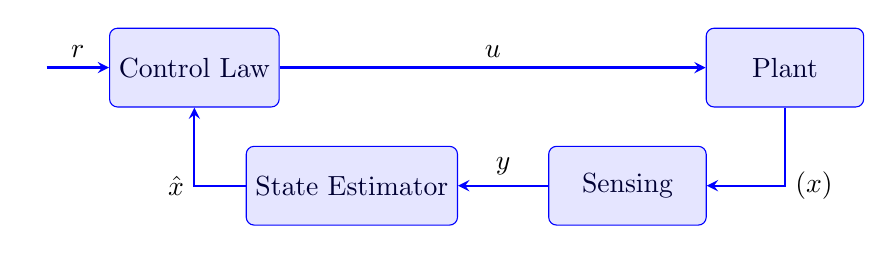
\begin{tikzpicture}[node distance=1.5cm]
    \node (in) [eNode] {};
    \node (control) [recNodeB, right of=in, xshift=0.5cm] {Control Law};
    \node (sys) [recNodeB, right of=control, xshift=6cm] {Plant};
    \node (sensor) [recNodeB, below of=sys, xshift=-2cm] {Sensing};
    \node (estimator) [recNodeB, below of=control, xshift=2cm] {State Estimator};
    
    \draw [arrowB] (in) -- node[above] { $r$} (control);
    \draw [arrowB] (control) -- node[above] { $u$} (sys);
    \draw [arrowB] (sys) |- node[right] { ($x$)} (sensor);
    \draw [arrowB] (sensor) -- node[above] { $y$} (estimator);
    \draw [arrowB] (estimator) -| node[left] { $\hat{x}$} (control);
    \end{tikzpicture}
  }
\def\myPerionTable{
  \begin{tabular}{|c c c|} 
      \hline
      Task & Period & Deadline \\ 
      \hline
      Check for obstacles & 10ms & 1.5ms \\ 
      %\hline
      Check GPS position & 10ms & 0.5ms \\
      Control Law & 2ms & 0ms \\
      \multicolumn{3}{|c|}{$\cdots$}\\
      \hline
  \end{tabular}
}

\frame{
  \frametitle{An control problem example}
  \begin{center}
      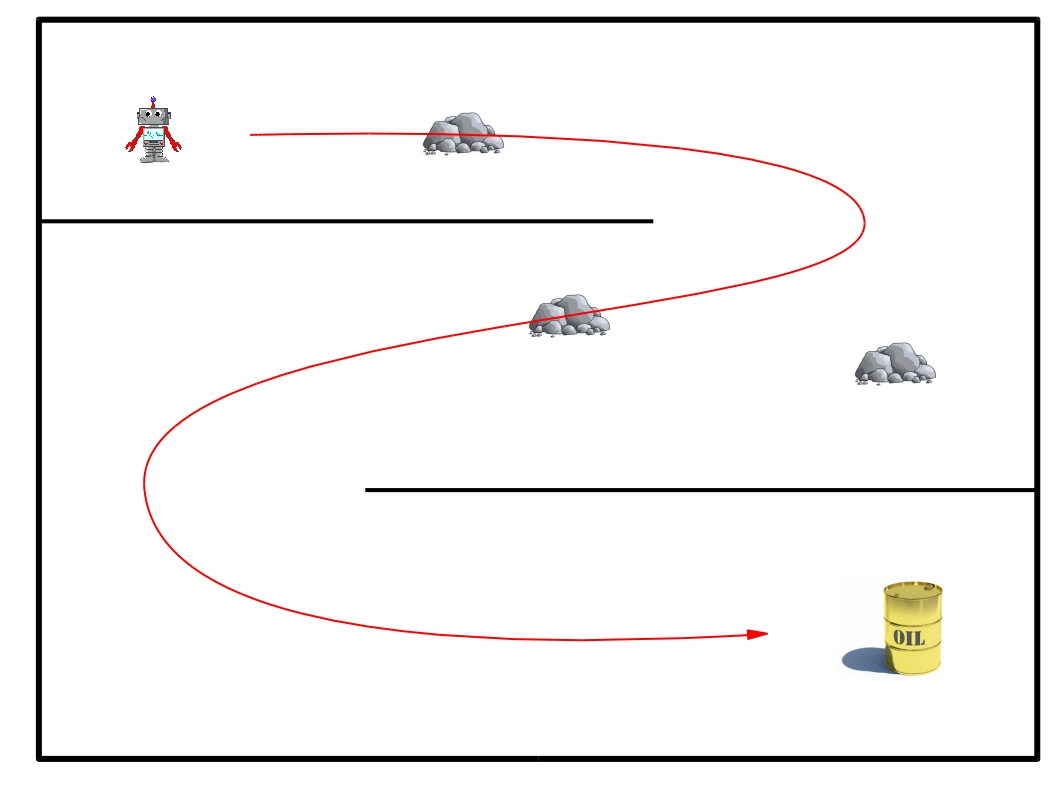
\includegraphics[width=80mm]{robotInMaze}
      
      Robot navigation
  \end{center}
}	
\frame{
    \frametitle{An control problem example}
    \begin{center}
        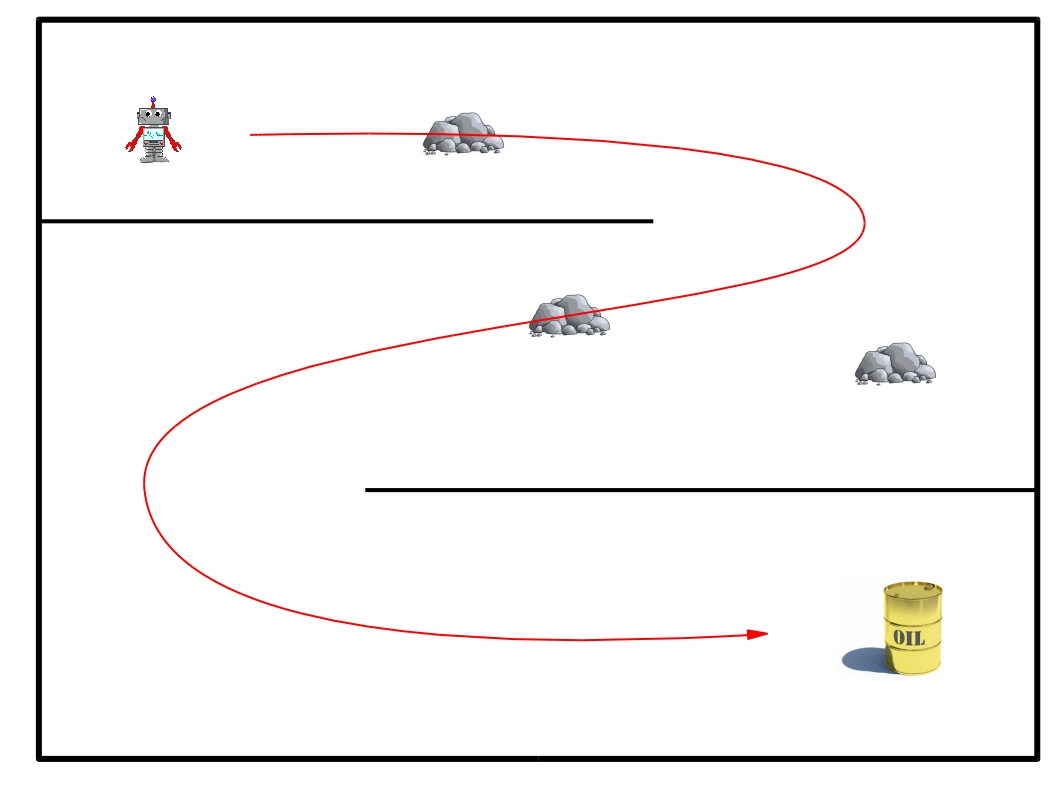
\includegraphics[width=50mm]{robotInMaze}
    \end{center}
    \begin{block}{The Objectives}
        \begin{itemize}
            \item The robot need to reach the target point \textbf{fast} and \textbf{safely}
            \item The robot have on-board camera for \textbf{obstacle-avoidance}
            \item The robot use GPS for general \textbf{navigating}
        \end{itemize}
    \end{block}
}	
\frame{
    \frametitle{The Traditional Solution}
    \begin{center}
        \tikzFeadback
    \end{center}
    \begin{center}
        {\Huge \textbf{+}}
    \end{center}
    \begin{block}{Constant time steps + periodic tasks}
        \begin{center}
            \todoil{{time steps\\ figure}} + 
            \myPerionTable
        \end{center}
    \end{block}
}	
\frame{
    \frametitle{The Main Software Design Problems}
    \begin{center}
        \myPerionTable
    \end{center}
    \begin{block}{The design problems from our point of view}
        \begin{itemize}
            \item \textbf{All the tasks are highly coupled}: \textit{any change or addition of some task require to consider all other tasks requirements}
            \item \textbf{Static and inefficient scheduling}: \textit{the table is defined for the worst case} \todoil{talk about related work on this direction}
            \item \textbf{No consideration of the environmental conditions}: it is a cyber-physical system after all
        \end{itemize}
    \end{block}
}  
\frame{
    \frametitle{The Goal}
    \begin{block}{}
        In this thesis we design an \textbf{reactive} scheduling framework for real-time systems
    \end{block}
    \begin{block}{Required features: \commentOut{of the scheduling framework for real-time systems}}
        \begin{itemize}
            \item \textbf{Independent} and \textbf{composable} requirements
            \item \textbf{Control objective based} requirement interface
            \item Environment \textbf{adoptive} scheduler
        \end{itemize}
    \end{block}
}

\subsection[Architecture]{Component-based Architecture}

\def\tikzArch{
    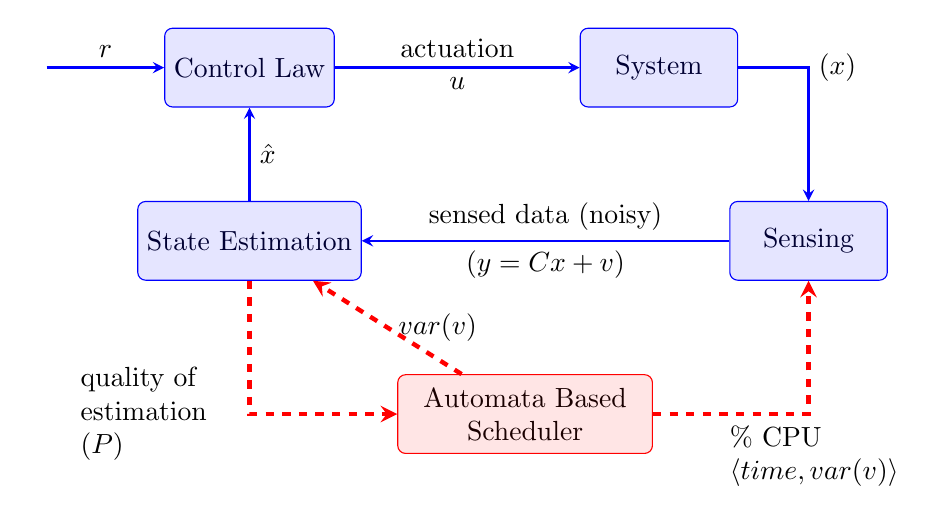
\begin{tikzpicture}[node distance=1.2cm]
    \node (in) [eNode] {};
    \node (control) [recNodeB, right of=in, xshift=1.5cm] {Control Law};
    \node (sys) [recNodeB, right of=control, xshift=4cm] {System};
    \node (sensor) [recNodeB, below of=sys, xshift=1.9cm, yshift=-1cm] {Sensing};
    \node (estimator) [recNodeB, below of=control, yshift=-1cm] {State Estimation};
    \node (sched) [recNodeG, below of=estimator, yshift=-1cm, xshift=3.5cm, text width=3cm] {Automata Based Scheduler};
    
    \draw [arrowB] (in) -- node[above] {$r$} (control);
    \draw [arrowB] (control) -- node[above] {actuation} node[below] {$u$} (sys);
    \draw [arrowB] (sys) -| node[right,text width=1cm] {($x$)} (sensor);
    \draw [arrowB] (sensor) -- node[above] {sensed data (noisy)} node[below] {$(y = Cx +v$)} (estimator);
    \draw [arrowB] (estimator) -- node[left,text width=2cm] {} node[right] {$\hat{x}$} (control);
    
    \draw [arrowG] (estimator) |- node[left,text width=2cm] {quality of estimation ($P$)} (sched);
    
    \draw [arrowG] (sched) -| node[below,text width=2cm] { \% CPU $\langle time,var(v) \rangle$} (sensor);
    %\draw [arrowG] (sched) -| node[right] {$\langle time,var(v) \rangle$} (sensor);
    
    \draw [arrowG] (sched) --  node[right] {$var(v)$} (estimator);
    
    \end{tikzpicture}
}
\def\AutoGeneral{
    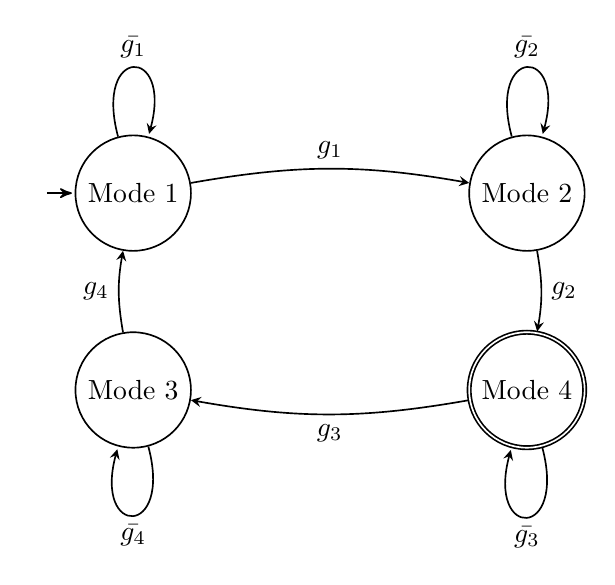
\begin{tikzpicture}[
        auto,
        semithick,
        >=stealth
        ]
        \node[state,initial](s0) {Mode 1};
        \node[state](s1) [right of=s0, xshift=4cm] {Mode 2};
        \node[state](s3) [below of=s0, yshift=-1.5cm] {Mode 3};
        \node[state, accepting](s2) [right of=s3, xshift=4cm] {Mode 4};
        \path[->]
        (s0) edge [loop above=10] node {$\bar{g_1}$} ()
        (s0) edge [bend left=10] node {$g_1$} (s1)
        (s1) edge [loop above] node {$\bar{g_2}$} ()
        (s1) edge [bend left=10] node {$g_2$} (s2)
        (s2) edge [loop below] node {$\bar{g_3}$} ()
        (s2) edge [bend left=10] node {$g_3$} (s3)
        (s3) edge [loop below] node {$\bar{g_4}$} ()
        (s3) edge [bend left=10] node {$g_4$} (s0)
        ;
    \end{tikzpicture}
}
\def\AutoCarObs{
    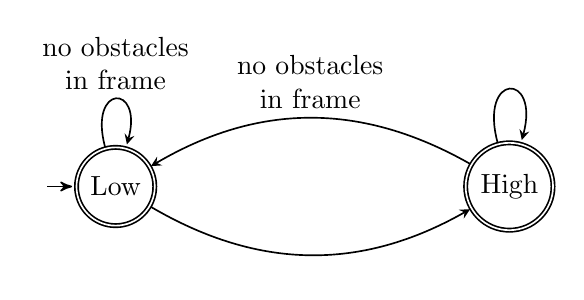
\begin{tikzpicture}[
    auto,
    semithick,
    >=stealth, text centered
    ]
    \node[state,initial, accepting](s0) {Low};
    \node[state,accepting](s1) [right of=s0, xshift=4cm] {High};
    \path[->]
    (s0) edge [loop above=10, text width=2cm] node {no obstacles in frame} ()
    (s0) edge [bend right] node {} (s1)
    (s1) edge [bend right, text width=2cm, above] node {no obstacles in frame} (s0)
    (s1) edge [loop above=10] node {} ()
    ;
    \end{tikzpicture}
}
\def\AutoCarGPS{
    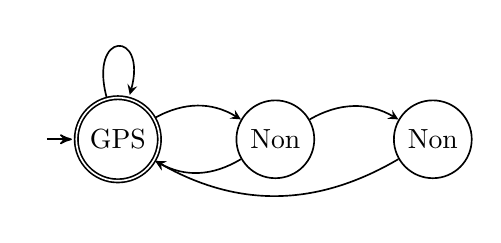
\begin{tikzpicture}[
    auto,
    semithick,
    >=stealth, text centered
    ]
    \node[state,initial,accepting](gps) {GPS};
    \node[state](s0) [right of=gps, xshift=1cm] {Non};
    \node[state](s1) [right of=s0, xshift=1cm] {Non};
    
    \path[->]
    (gps) edge [loop above=10, text width=2cm] node {} ()
    (s0) edge [bend left] node {} (gps)
    (s1) edge [bend left] node {} (gps)
    
    (gps) edge [bend left] node {} (s0)
    (s0) edge [bend left] node {} (s1)
    
    ;
    \end{tikzpicture}
}
\def\AutoCarComp{
    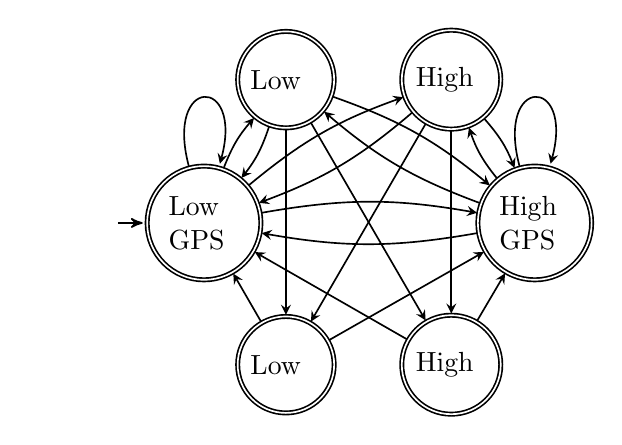
\begin{tikzpicture}[
    auto,
    semithick,
    >=stealth,
    text width=0.9cm
    ]
    \node[state,initial,accepting](s0) at (2.46,2.6){Low GPS};
    \node[state,accepting](s1) at (3.5,4.42){Low};
    \node[state,accepting](s2) at (5.6,4.42){High};
    \node[state,accepting](s3) at (6.66,2.6){High GPS};
    \node[state,accepting](s4) at (5.6,0.8){High};
    \node[state,accepting](s5) at (3.5,0.8){Low};
    \path[->]
    (s0) edge [loop above] node {} ()
    (s0) edge [bend left=10] node {} (s1)
    (s0) edge [bend left=10] node {} (s2)
    (s0) edge [bend left=10] node {} (s3)
    (s1) edge [bend left=10] node {} (s0)
    (s1) edge [bend left=10] node {} (s3)
    (s1) edge [] node {} (s4)
    (s1) edge [] node {} (s5)
    (s2) edge [bend left=10] node {} (s0)
    (s2) edge [bend left=10] node {} (s3)
    (s2) edge [] node {} (s4)
    (s2) edge [] node {} (s5)
    (s3) edge [bend left=10] node {} (s0)
    (s3) edge [bend left=10] node {} (s1)
    (s3) edge [bend left=10] node {} (s2)
    (s3) edge [loop above] node {} ()
    (s4) edge [] node {} (s0)
    (s4) edge [] node {} (s3)
    (s5) edge [] node {} (s0)
    (s5) edge [] node {} (s3)
    ;
    \end{tikzpicture}   
}
\def\AutoCarObsGameBased{
    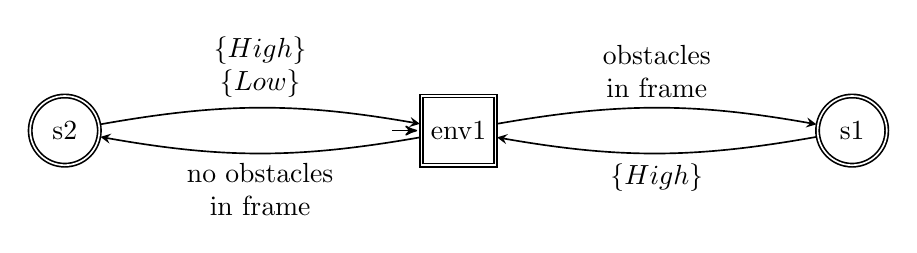
\begin{tikzpicture}[
        auto,
        semithick,
        >=stealth,
        ,text centered,
        p0/.style={circle},p1/.style={rectangle}
        ]
        \node[state,accepting,p0](s1) {s2};
        \node[state,initial,accepting,p1, right of=s1, xshift=4cm](s2) {env1};
        \node[state,accepting,p0, right of=s2, xshift=4cm](s3){s1};
        \path[->]
        (s1) edge [bend left=10, text width=2cm] node {$\left\{ High \right\}$ $\left\{ Low \right\}$} (s2)
        (s2) edge [bend left=10, text width=2cm] node {no obstacles in frame} (s1)
        (s2) edge [bend left=10, text width=2cm] node {obstacles in frame} (s3)
        (s3) edge [bend left=10] node {$\left\{ High \right\}$} (s2)
        ;
    \end{tikzpicture}
}

\frame{
    \frametitle{The Proposed Architecture}
    
    %\begin{center}
    \begin{columns}
        \begin{column}{5cm}
            \scalebox{0.5}{
                \tikzArch
            }
        \end{column}
        \hfill
        {\huge +}
        \hfill
        \begin{column}{4cm}
            \scalebox{0.5}{
                \AutoGeneral
            }
        \end{column}
    \end{columns}
    %\end{center} 
}
\frame{
    \frametitle{System Design}
    \framesubtitle{The Proposed Architecture}
    \todoil{Explain that the scheduler is involve in the control loops}
    \begin{center}
        \scalebox{0.9}{
            \tikzArch
        }
    \end{center} 
}
\frame{
    \frametitle{Automata-Based Specification Interface}
    \framesubtitle{The Proposed Architecture}
    \todoil{maybe add a word about RTcomposer and GameComposer}\\
    \begin{center}
        \scalebox{0.4}{
            \AutoGeneral
        }
    \end{center} 
    
    \begin{block}{Why Automata}
        \begin{itemize}
            \item \textbf{Lite:} minimal resource consumption at run-time
            \item \textbf{Composable}: easy to compose independent components
            \item \textbf{Automata theory built in:} allows for tools such \emph{GOAL}
            \item \textbf{Expressiveness}
        \end{itemize}
    \end{block}
}
\frame{
    \frametitle{Example of Guarded Automata}
    \framesubtitle{The Proposed Architecture}
    \begin{center}
        \begin{columns}
            \begin{column}{5cm}
                \begin{block}{Obstacle avoidance component}
                    \centering
                    \scalebox{0.6}{
                        \AutoCarObs
                    }
                \end{block}
                \begin{block}{GPS navigation component}
                    \centering
                    \scalebox{0.6}{
                        \AutoCarGPS
                    }
                \end{block}
            \end{column}
            %\hfill
            {\Huge $\Rightarrow$}
            %\hfill
            \begin{column}{5.5cm}
                \begin{block}{Composed guarded automata}
                    %\centering
                    \scalebox{0.65}{
                        \AutoCarComp
                    }
                \end{block}
            \end{column}
        \end{columns}
    \end{center}
}
\frame{
    \frametitle{Simplifying the Guarded Automata}
    \framesubtitle{The Proposed Architecture}
    
    
    \begin{block}{Mode-based guarded automata (for good intuition)}
        \centering
        \scalebox{0.6}{
            \AutoCarObs
        }
    \end{block}
    
    %\begin{center}
        { $\Downarrow$}
    %\end{center}
    
    \begin{block}{The automata in practice (best match $\omega$-word theory)}
        \centering
        \scalebox{0.7}{
            \AutoCarObsGameBased
        }
    \end{block}
    \textbf{Q: How to create the guarded automata?} By wining \buchi games
}

\subsection[\buchi Games]{\buchi Games Interface}
\frame{
    \frametitle{\buchi game remainder}
    \begin{center}
            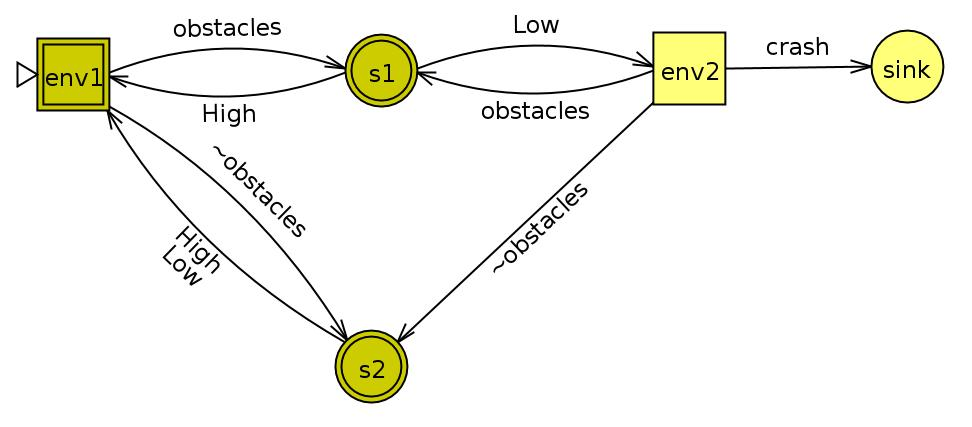
\includegraphics[width=90mm]{carObsGame.jpg}
    \end{center}    
}
\frame{
    \frametitle{\buchi game remainder}
    \begin{center}
            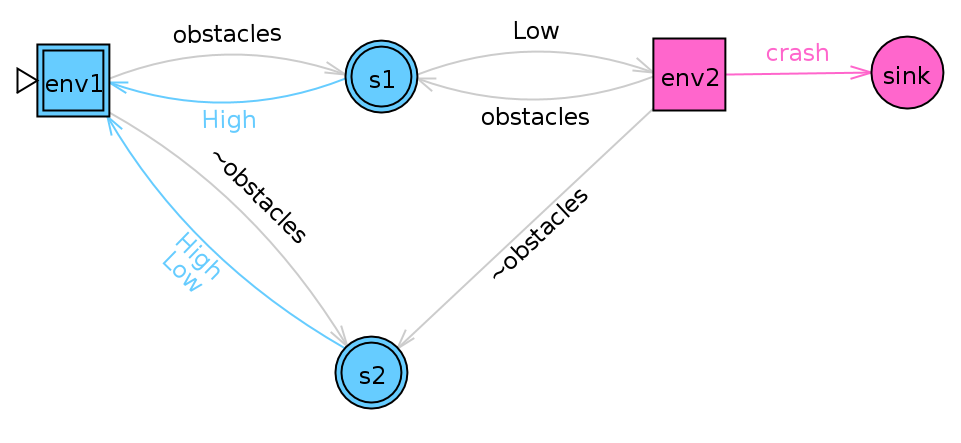
\includegraphics[width=90mm]{carObsGameStrategy}
    \end{center}    
}

%TODO \subsection[Component Definition]{Sub-Summery: Component Definition}
\frame{ %component definition
    \frametitle{A Component in the System}
    \begin{center}
            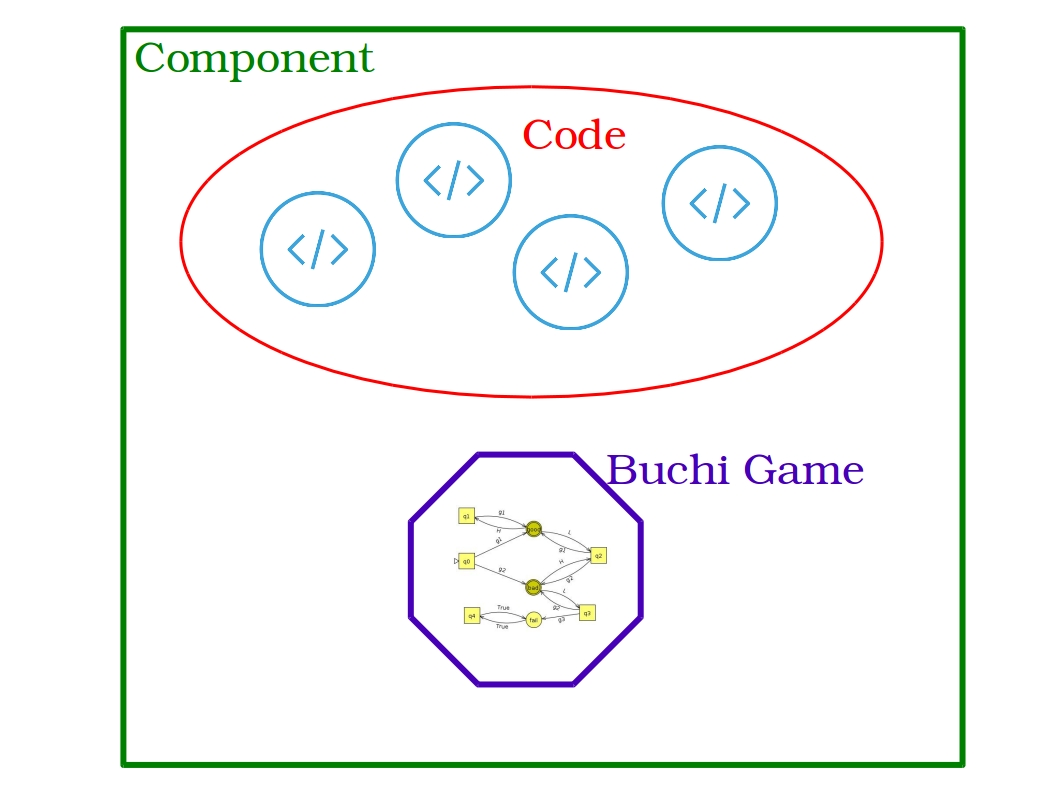
\includegraphics[width=60mm]{componentBase}
    \end{center}
    \begin{block}{Component Definition ($\langle T,G \rangle$)}
        \begin{itemize}
            \item A set of subroutines (functions code)
            \item A Generalize \buchi Game
        \end{itemize}
    \end{block}
}
\frame{
    \frametitle{A Component in the System}
    \begin{center}
        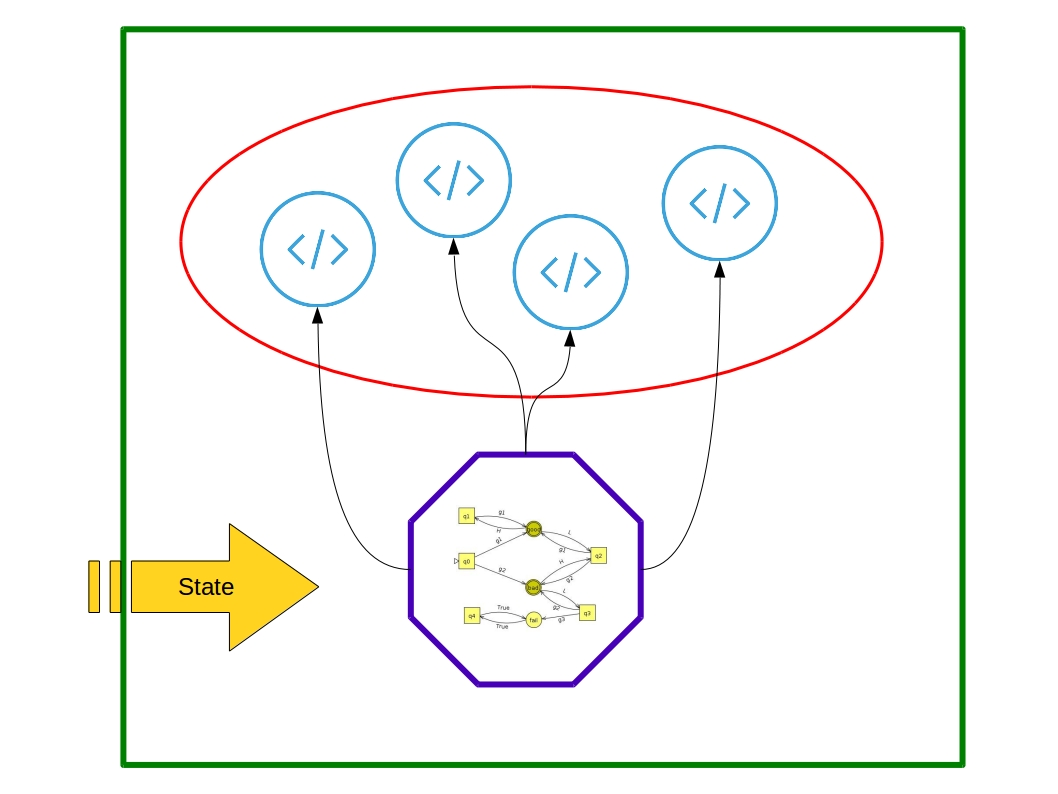
\includegraphics[width=60mm]{component}
    \end{center}
    \begin{block}{The \buchi game ($G=\langle A , \langle P_{sched} , P_{env} \rangle \rangle$)}
        \begin{itemize}
            \item Is played in turns by the \textbf{environment} and the \textbf{scheduler}
            \item Represent the \textbf{interaction} between the scheduler and the environment reaction
        \end{itemize}
    \end{block}
}
\frame{
    \frametitle{Scheduling \buchi Game}
    \framesubtitle{A Component in the System}
    
    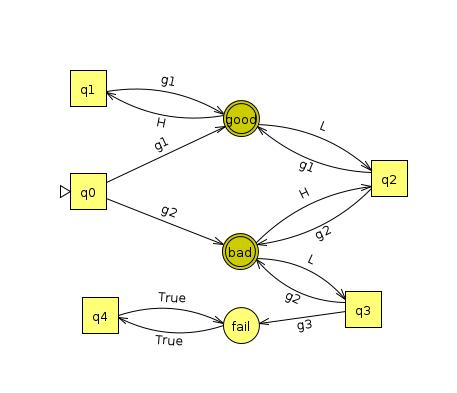
\includegraphics[width=30mm]{gameExample}
    
    \begin{block}{Scheduling \buchi Game}
        \begin{itemize}
            \item \textbf{Alternating turns}
            \item Scheduler alphabet is $\Sigma_{schd} = 2^T$
            \item Environment alphabet is $\Sigma_{env} = \mathbb{R}^n$ {\tiny (\textit{scheduler feedback variables})}
            \item There is an Edge for any \textbf{possible} environmental outcome 
            \item The \textbf{scheduler feedback variables} can be any environment-depended value
            \item Environment player plays first
        \end{itemize}
    \end{block}
}
\frame{ % game example
    \frametitle{Example - \buchi Game}
    \framesubtitle{A Component in the System}
    {The \buchi Game of the obstacles avoidance component:}
    
    \begin{center}
        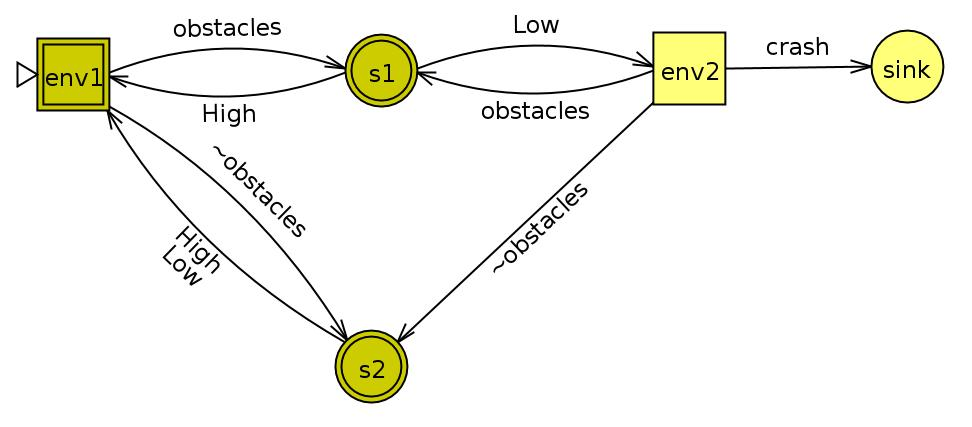
\includegraphics[width=80mm]{carObsGame}
    \end{center}
    
    \begin{block}{}
        \begin{itemize}
            \item The objectives of the component is to avoid obstacles
            \item The scheduler \textbf{win} $\Leftrightarrow$ the corresponding word $\omega \in \L(A)$ $\Leftrightarrow$ the component achieved his \textbf{objectives}
        \end{itemize}
    \end{block}
}
\frame{ % composition
    \frametitle{Component Composition}
    \begin{center}
        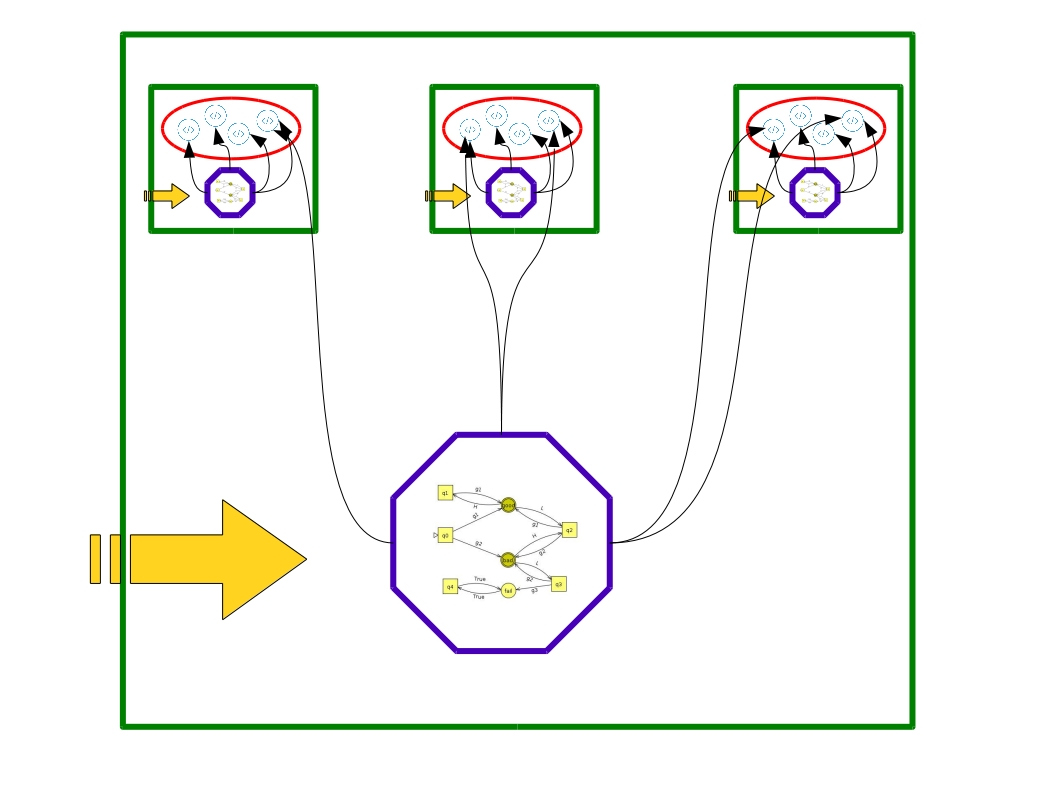
\includegraphics[width=100mm]{componentComp}
    \end{center}
}
\frame{
    \frametitle{Component Composition}
    \begin{center}
        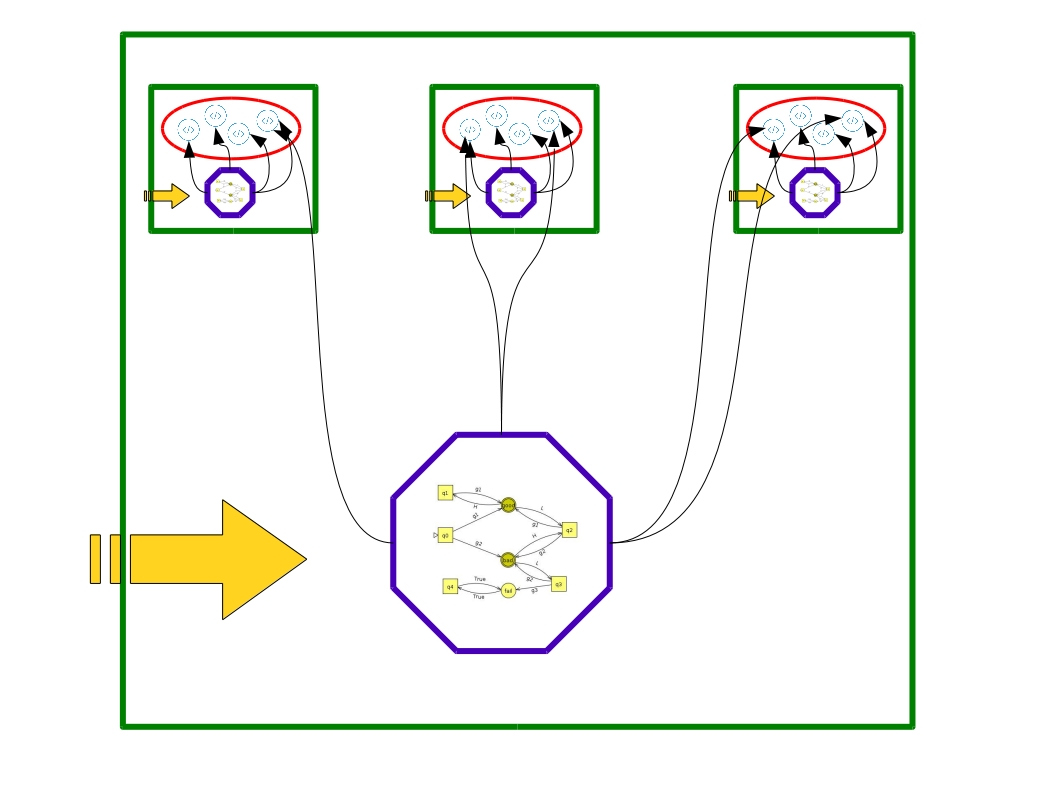
\includegraphics[width=40mm]{componentComp}
    \end{center}
    
    \begin{block}{Requirements}
        \begin{itemize}
            \item A game ($G=\langle A , \langle P_{s} , P_{e} \rangle \rangle$) correspond to all the components
            \item The game of Component is $G_i=\langle A_i , \langle P^i_{s} , P^i_{e} \rangle \rangle$
            \item $\omega \in \L(A) \Leftrightarrow \forall i : \omega(i) \in \L(A_i)$ 
        \end{itemize}
    \end{block}
}
\frame{
    \todoil{TODO: how to present the composition details?}\\
}
\frame{
    \todoil{TODO: show the resource component}\\
}
\frame{
    \todoil{TODO: show the scheduler work: 1. find wining strategy 2. simultaneously walk through the strategy automata}\\
}

    
\section[Kalman Filter]{Integration with Kalman}
\subsection{Guiding Concept}
\frame{
    \frametitle{Integration with Kalman}
    
    \begin{center}
        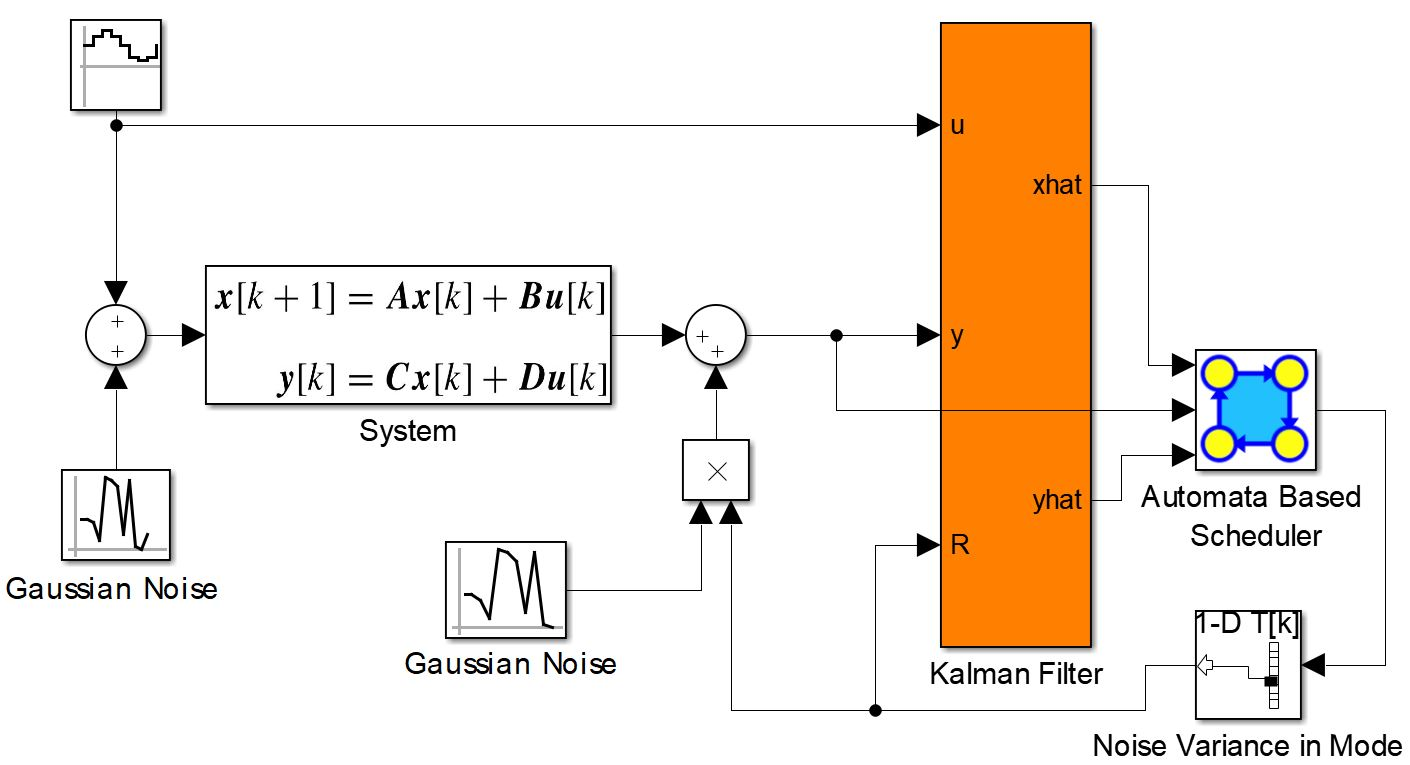
\includegraphics[width=40mm]{SimulinkModel}
        \hfill
        %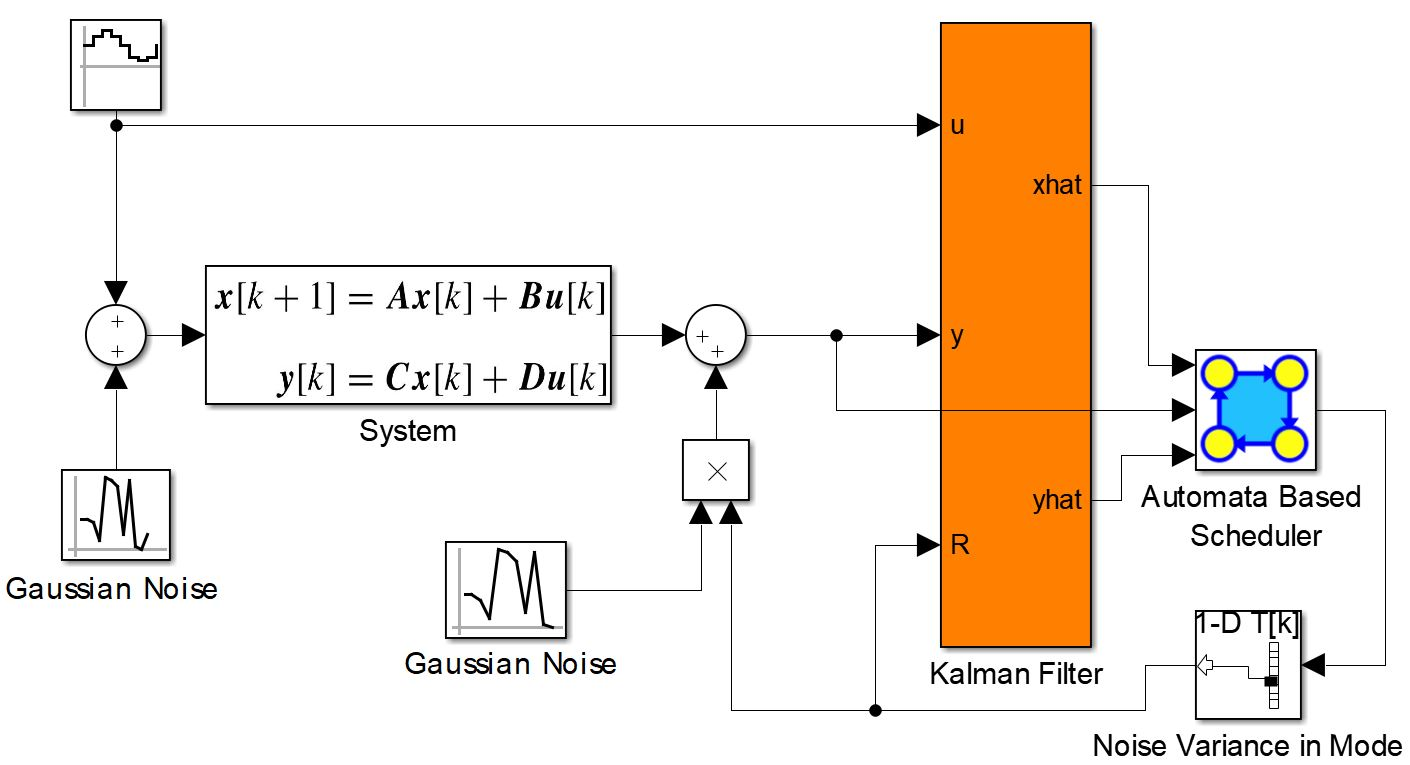
\includegraphics[width=40mm]{SimulinkModel}
        \todoil{Kalman filter figure}
    \end{center}

    \begin{block}{Resource utilization with Kalman filter}
        \begin{itemize}
            \item Novel technique for on-line trade-off between estimation quality and resource consumption
            \item Evaluate the overall errors using Kalman filter
            \item Schedule sensing-tasks based on the estimation quality
        \end{itemize}
    \end{block}
}
\frame{
    \frametitle{Integration with Kalman}
    \todoil{Explain the concept of estimate the errors}
    
    \begin{center}
        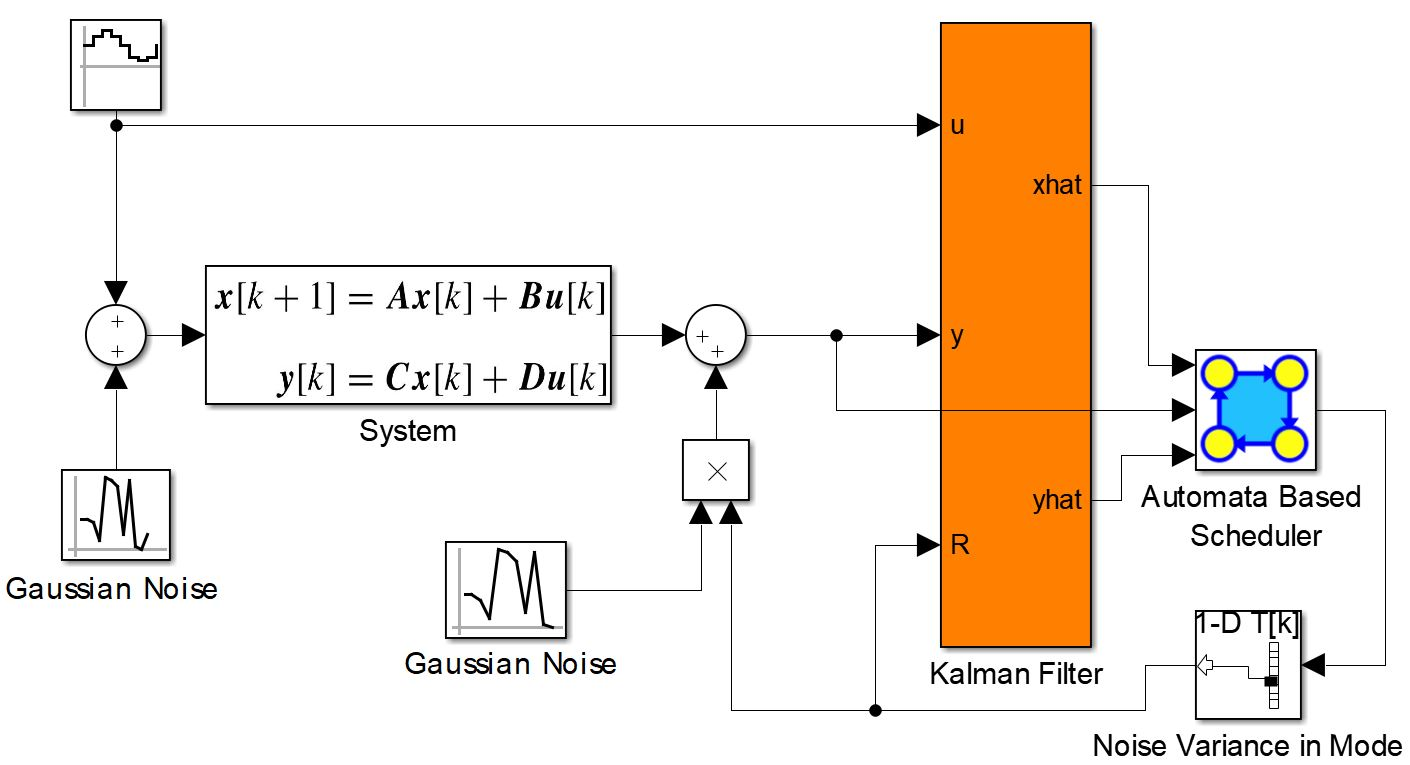
\includegraphics[width=40mm]{SimulinkModel}
    \end{center}
}
   
\subsection{Guided Tour Simulation}

\frame{
    \todoil{TODO}
}

\section[Experiment]{Experiment with real-life case-study}
\subsection{The Mission}
\frame{
    \frametitle{Mission Definition}
    \todoil{Explain the window motivation}
    \begin{center}
        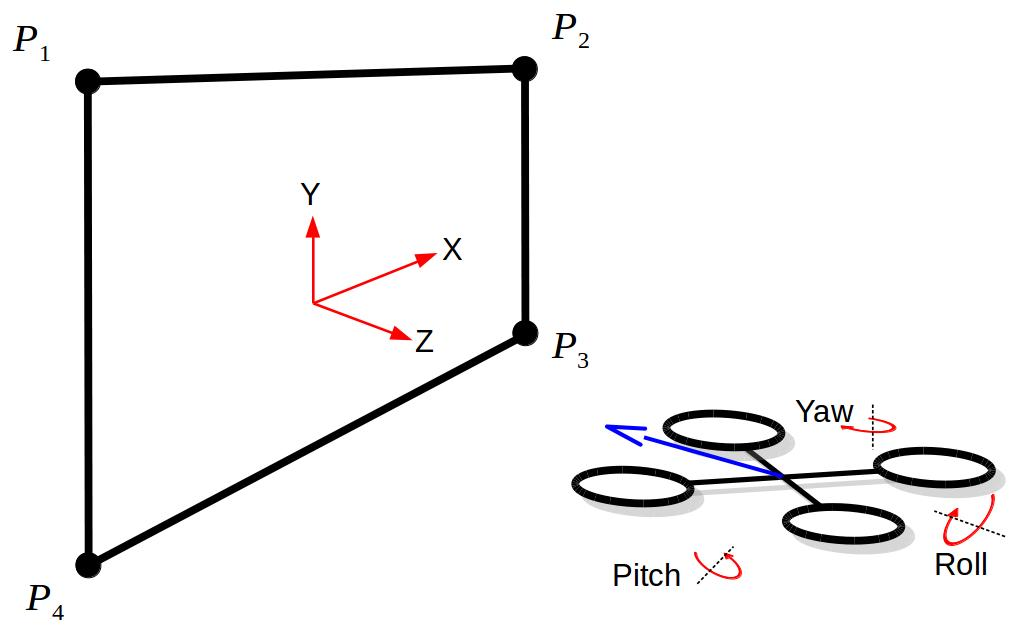
\includegraphics[width=100mm]{axis}
    \end{center}
}
\frame{
    \frametitle{Concrete Control Objectives}
    \begin{center}
        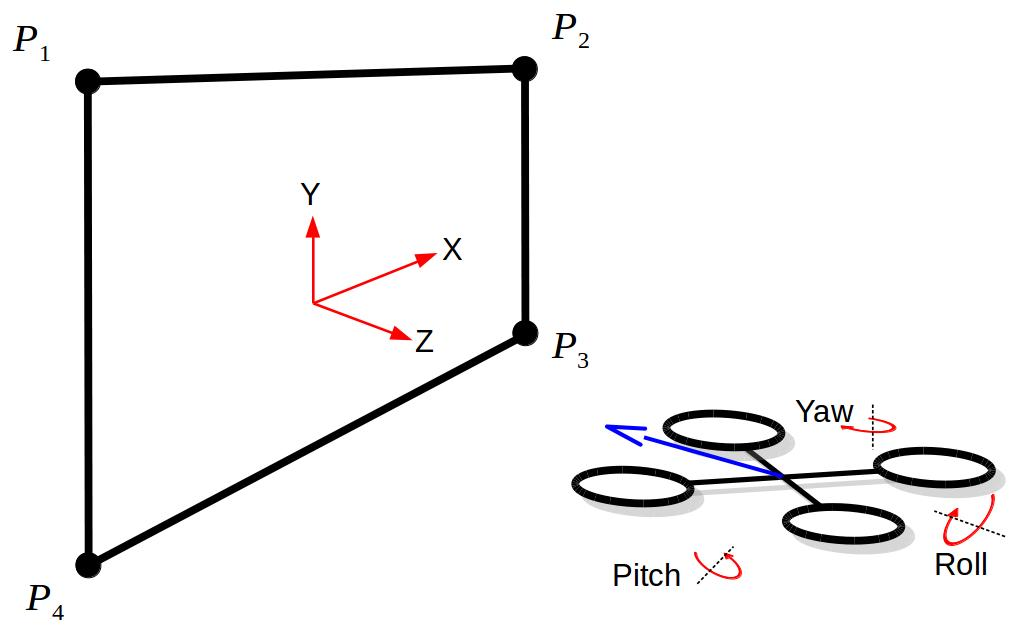
\includegraphics[width=70mm]{axis}
    \end{center}
    \begin{block}{ Control \& Scheduling Objectives }
        \begin{itemize}
            \item Minimize the $x$-deviation
            \item Minimize the CPU usage of image processing task
        \end{itemize}
    \end{block}
}
\frame{
    \frametitle{Traditional Controller Design}
    \begin{center}
        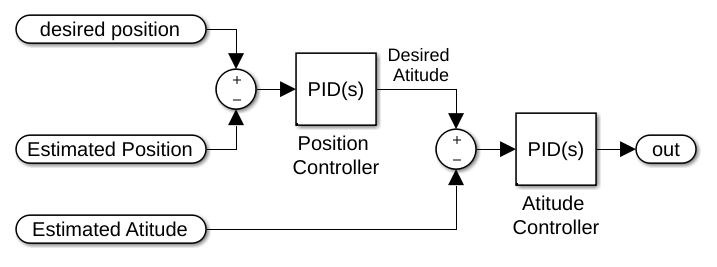
\includegraphics[width=90mm]{two_level_controller}
    \end{center}
    \begin{block}{ Attitude and position controller }
        \begin{itemize}
            \item \textbf{vision} component estimate the $x$-position
            \item Position controller output a desired roll angle
            \item Attitude controller is a traditional attitude controller
        \end{itemize}
    \end{block}
}

\subsection{Vision Component}
\frame{
    \frametitle{Vision Component}
    \begin{center}
        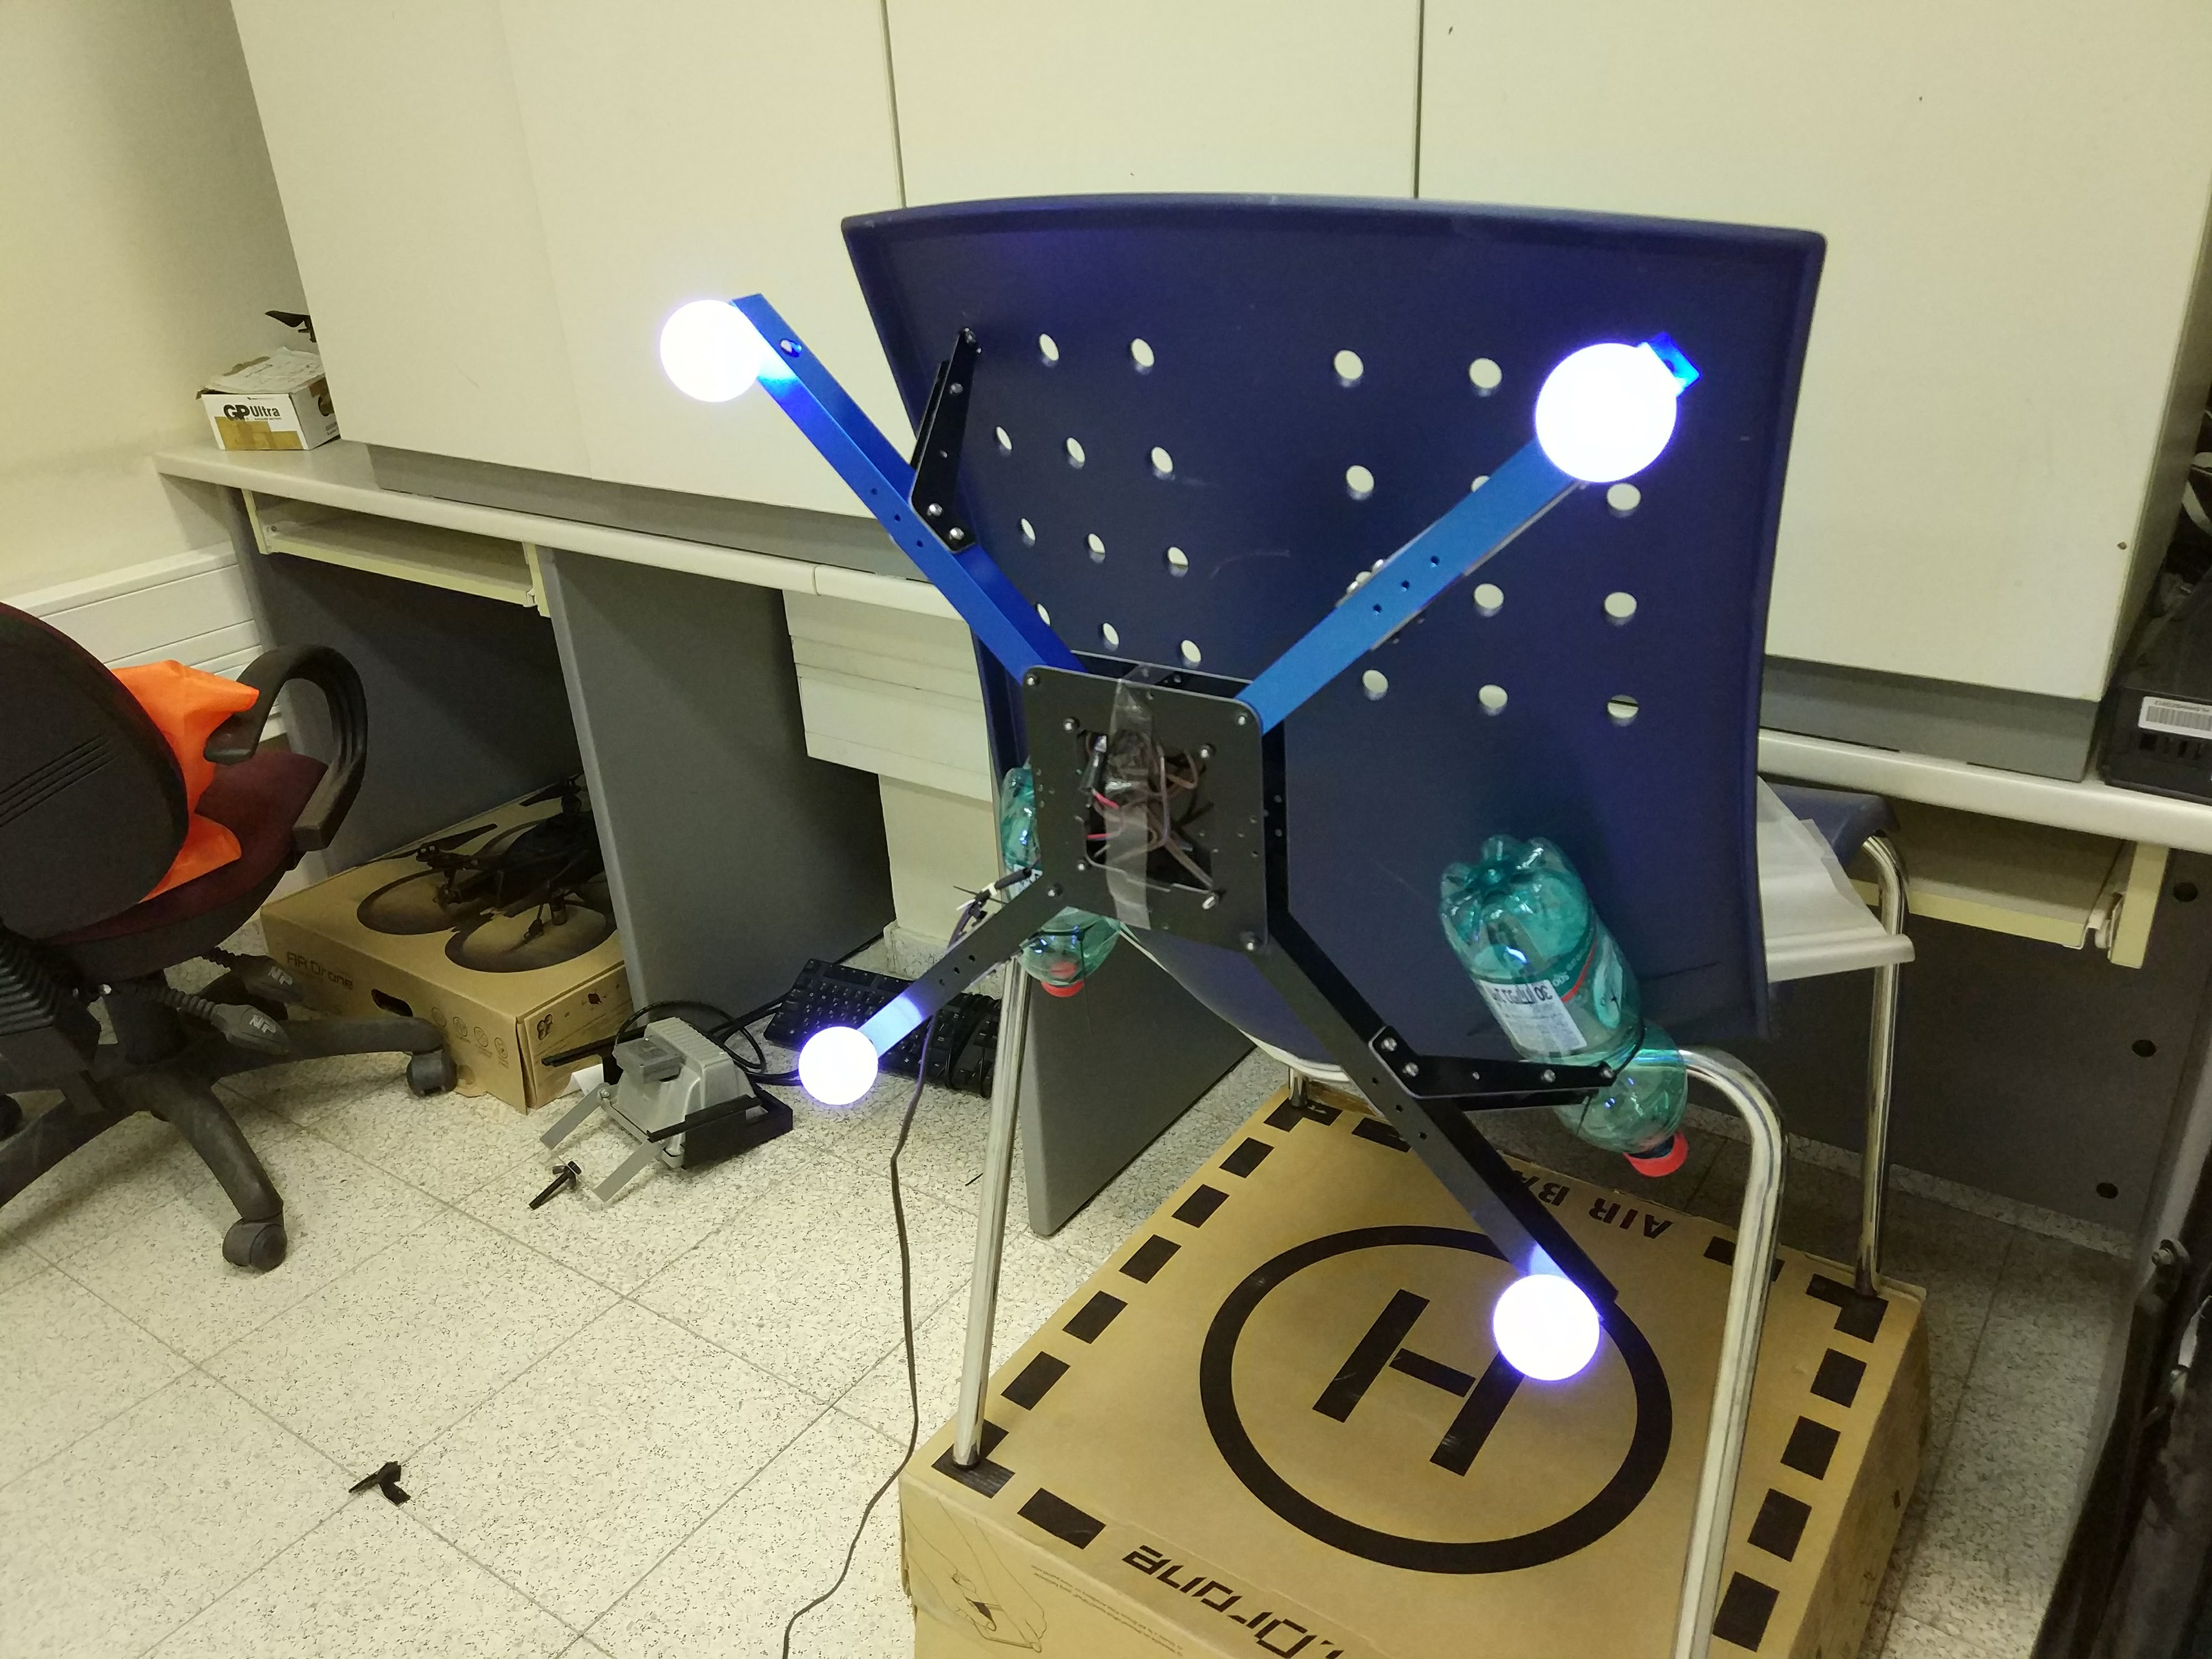
\includegraphics[width=60mm]{window_lights}
    \end{center}
    \begin{block}{ Image Processing Algorithm }
        \begin{enumerate}
            \item Find the window corners (brute force search)
            \item Calculate the drone position
        \end{enumerate}
    \end{block}
}
\frame{
    \frametitle{Calculate the Drone Position}
    \framesubtitle{Vertical Difference}
    \begin{center}
        \todoil{take a picture}
        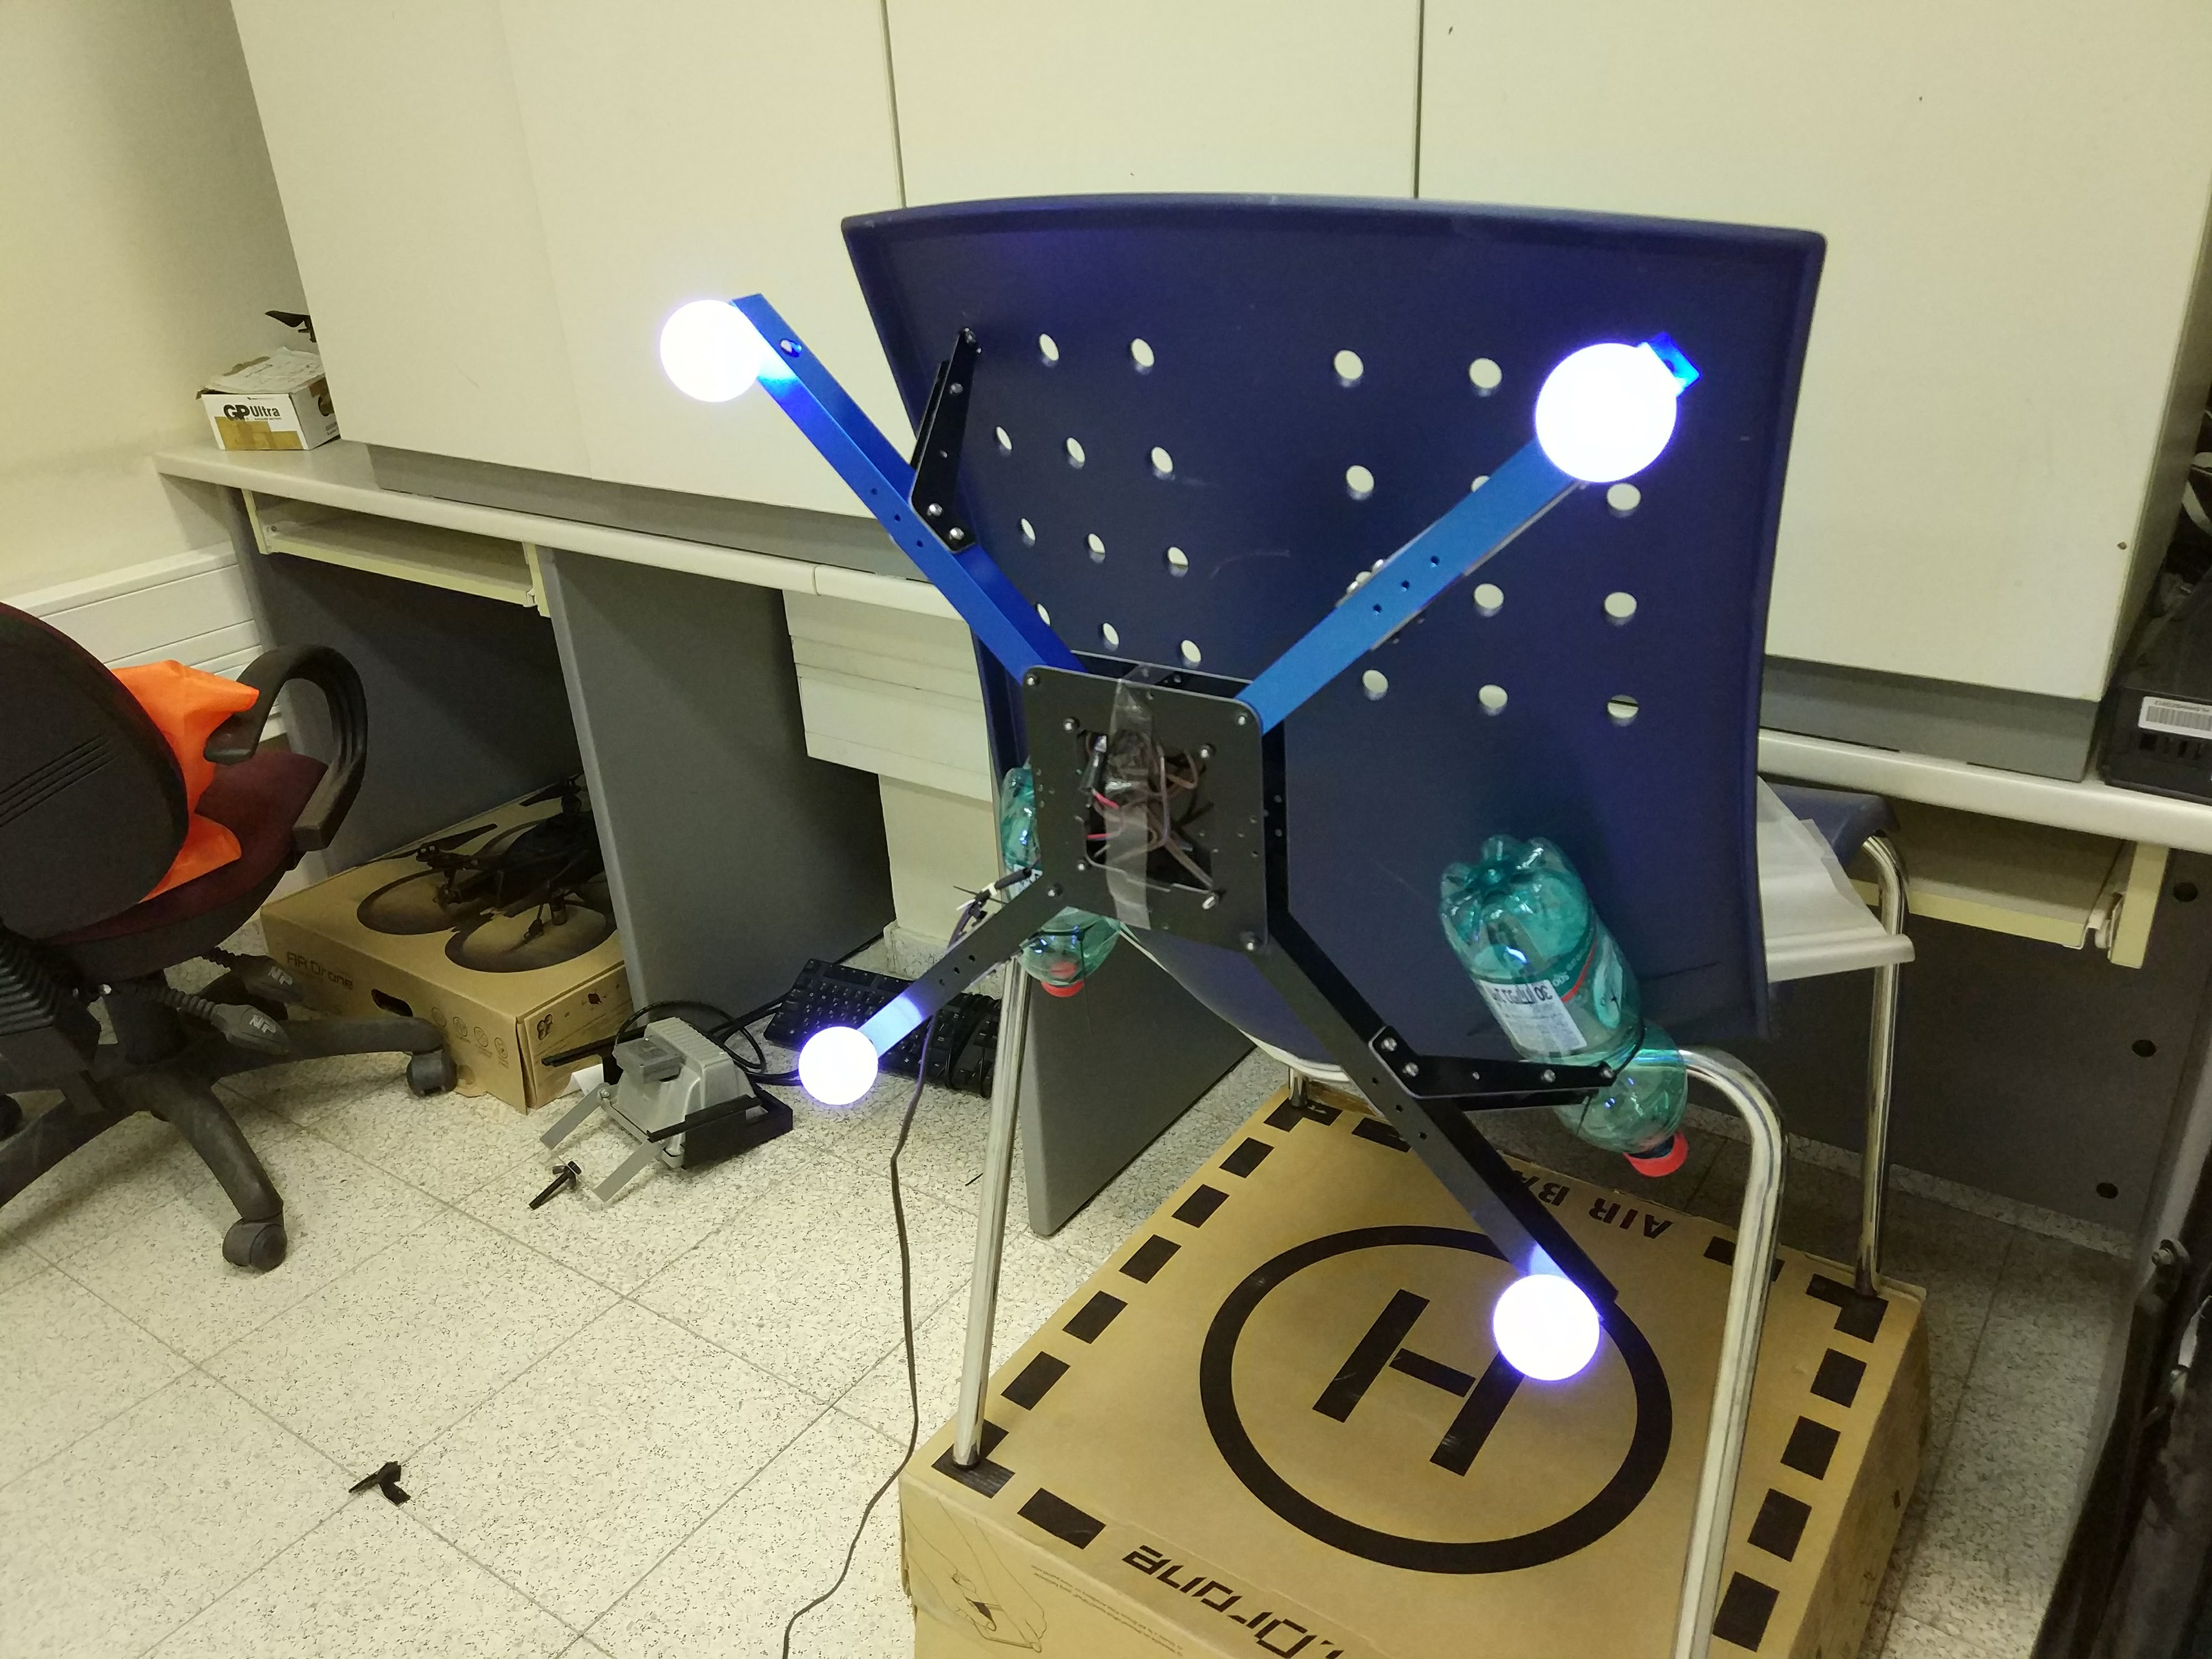
\includegraphics[width=60mm]{window_lights}
    \end{center}
    \begin{block}{ }
        \centering \Large $V_d = \frac{((y_1-y_4)-(y_2-y_3))}{((y_1-y_4)+(y_2-y_3))}$
    \end{block}
}
\frame{
    \frametitle{Calculate the Drone Position}
    \framesubtitle{Center of Mass}
    \begin{center}
        \todoil{take a picture}
        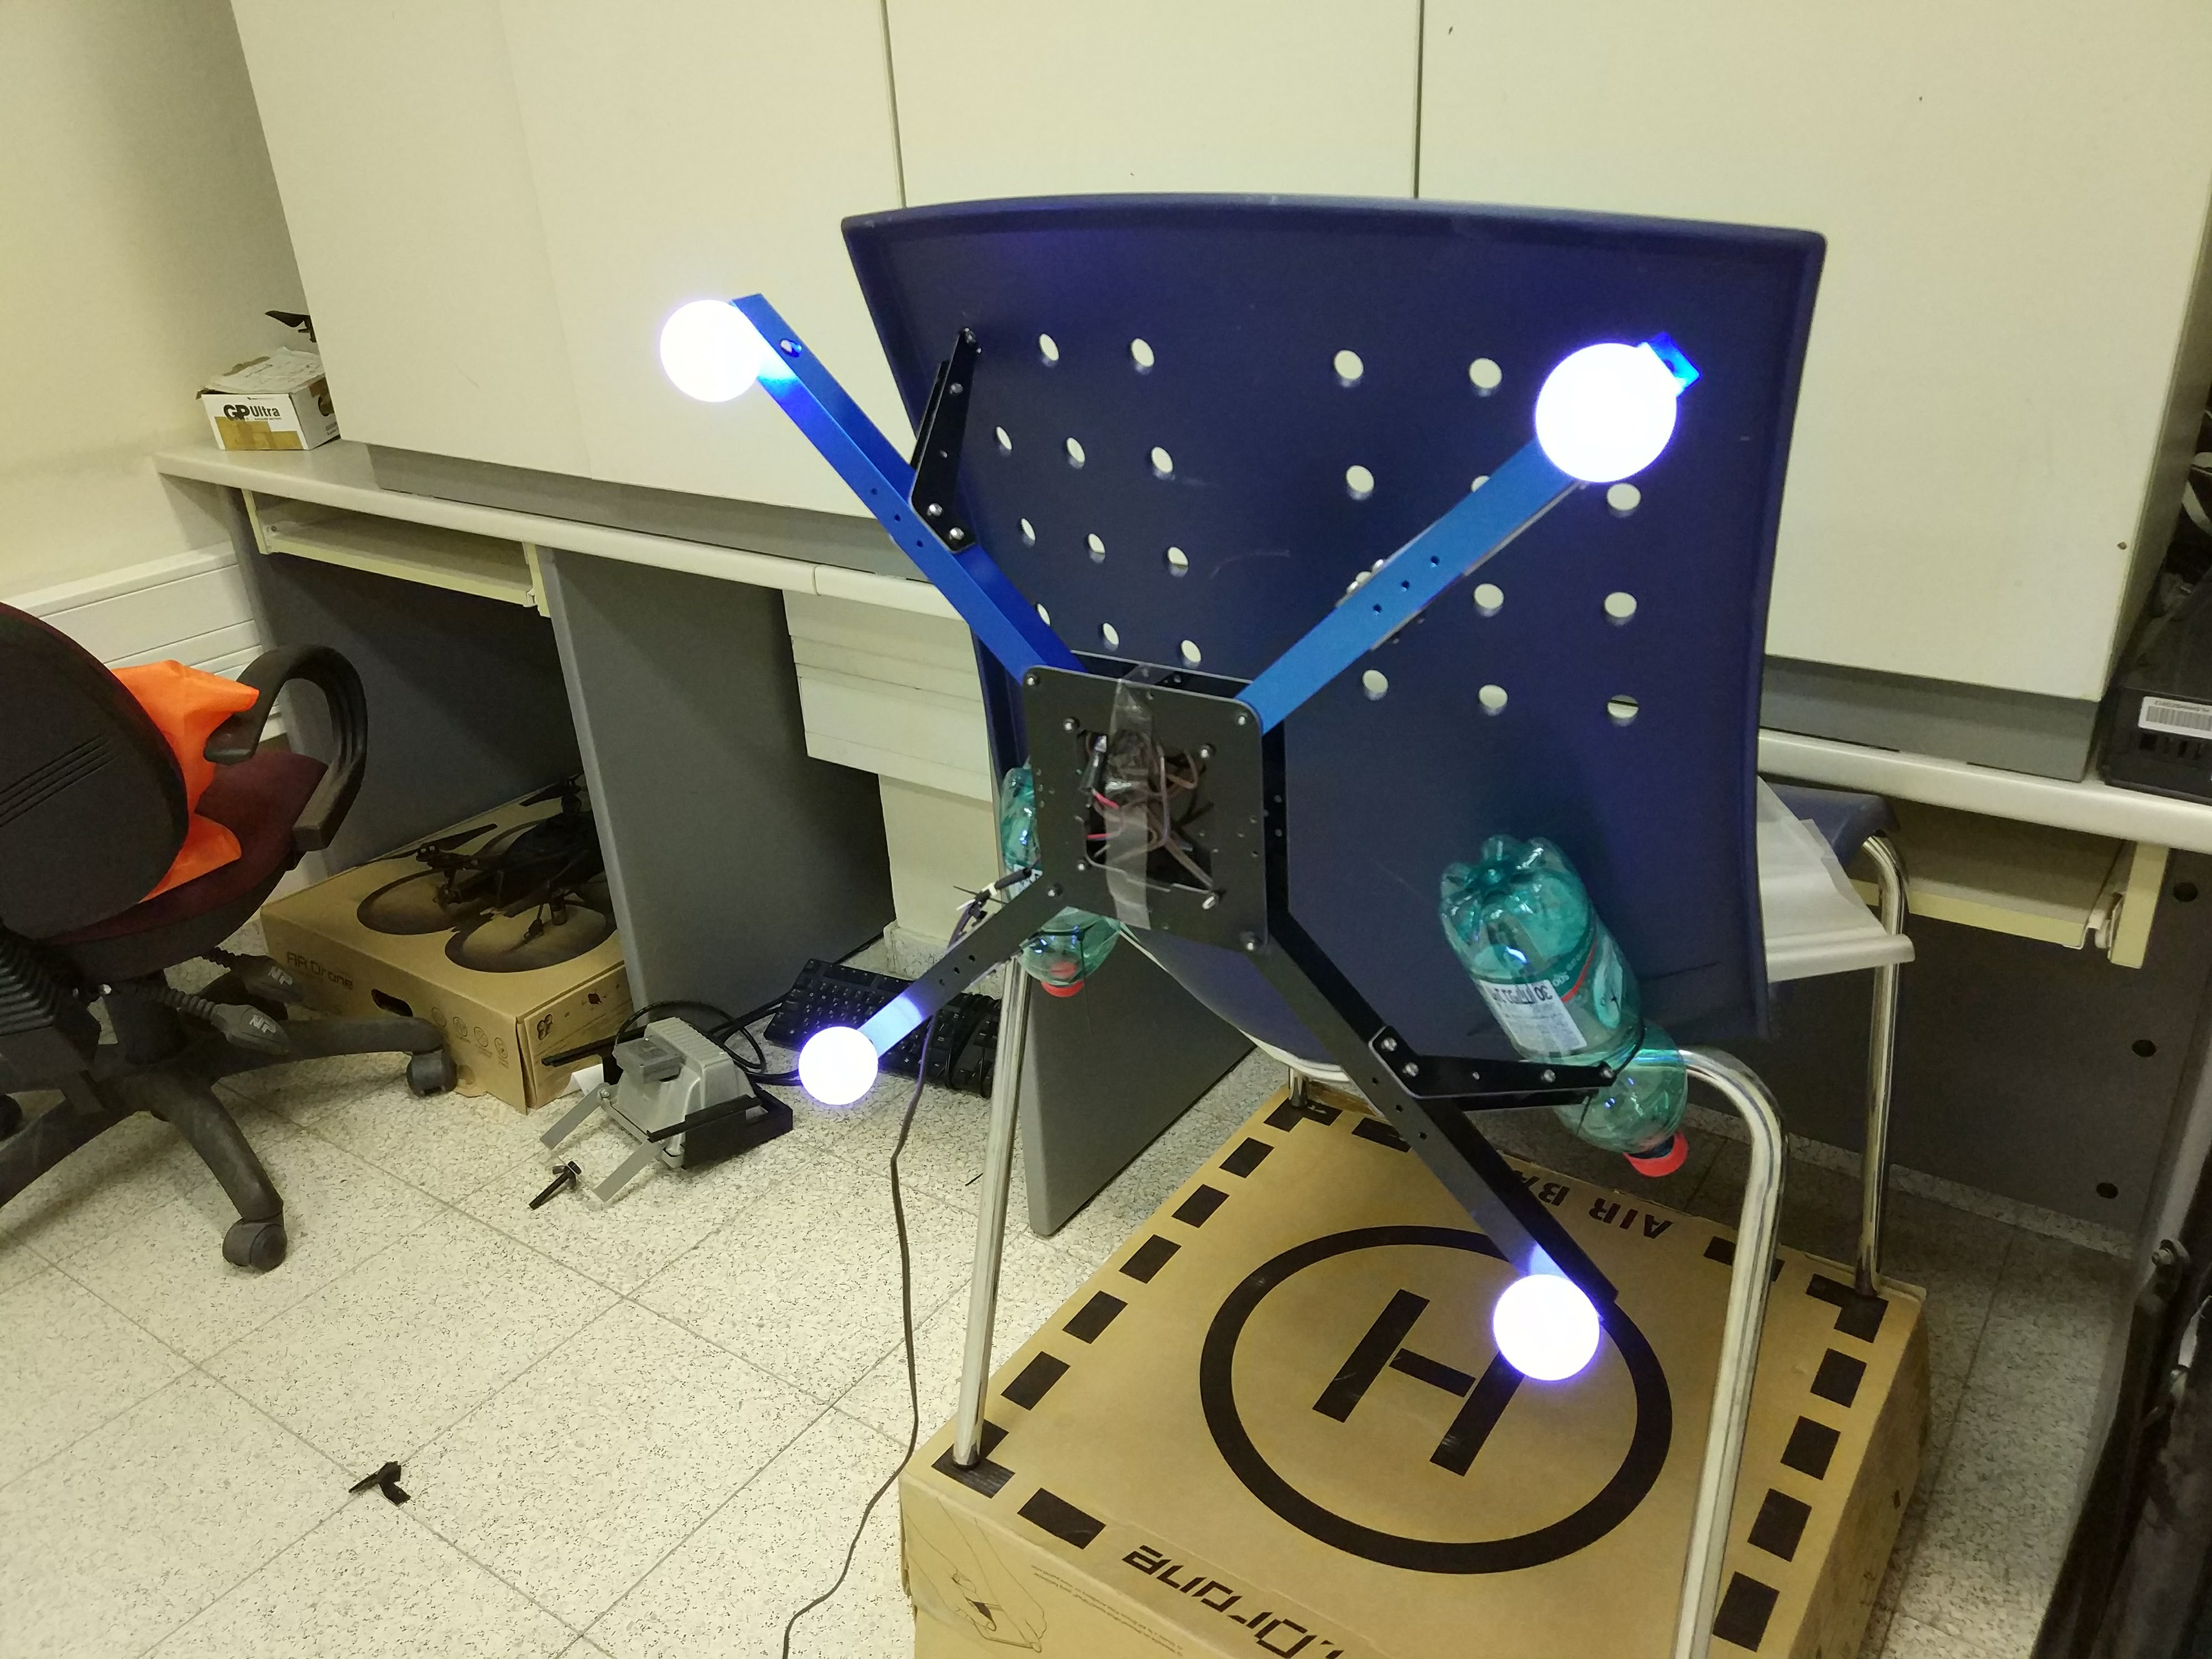
\includegraphics[width=60mm]{window_lights}
    \end{center}
    \begin{block}{ }
        \centering \Large $S_x = \frac{x_1 + x_2 + x_3 + x_4}{4}$
    \end{block}
}
\frame{
    \frametitle{Calculate the Drone Position}
    \begin{center}
        \todoil{take a picture}
        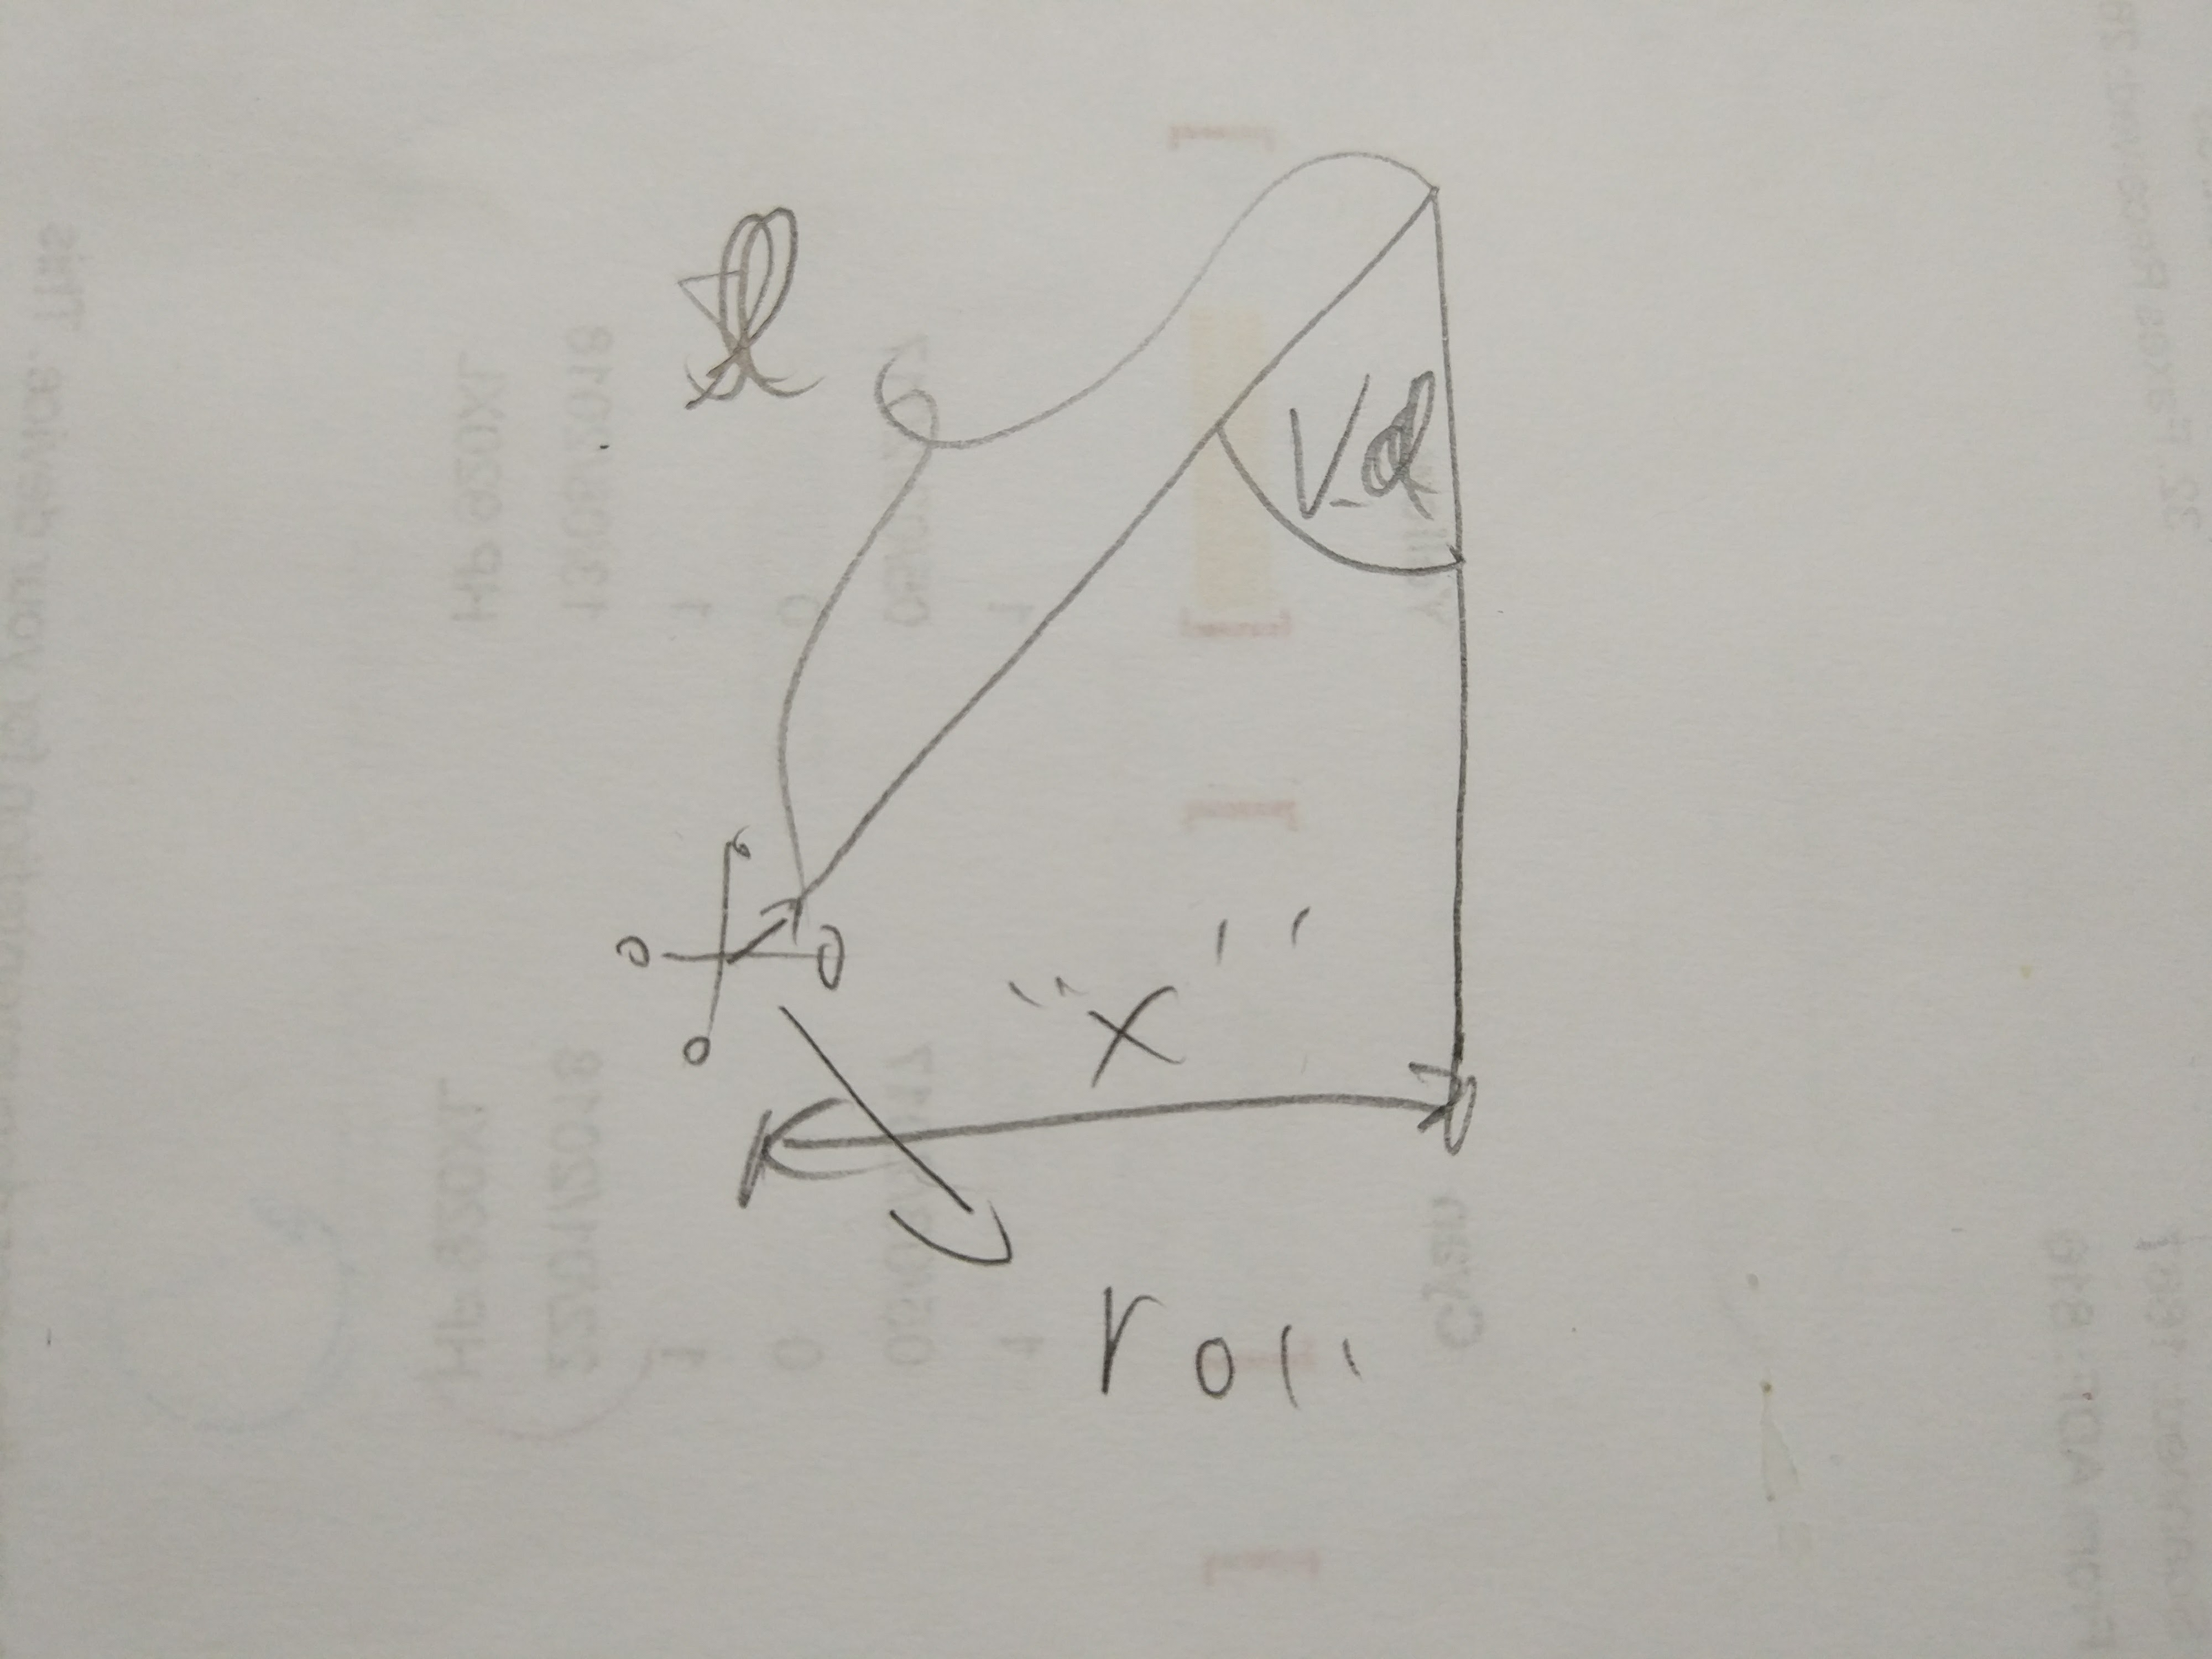
\includegraphics[width=50mm]{vd-geometry}
    \end{center}
    \begin{block}{ }
        $x = l \cdot \sin(V_d) \approx l \cdot V_d$
    \end{block}
}

\subsection[complementary filter]{Simplifying the Kalman filter with complementary filter}
    \todoil{1. why not Kalman}
    \todoil{2. how we use complementary filter}
    \todoil{3. the linearize model in $x$ / roll axis}
    \todoil{4. update state (equations)}
\subsection{Results}
    \todoil{the automata and their results}


% % % % Conclusion  % % % %
% % % % % % % % % % % % % %
\section{Conclusion}
\subsection{Conclusion}
    \todoil{instead of with Related Work}
\subsection{Related Work}
    \todoil{review of similar papers: A table with few papers}
\frame{
%        \frametitle{Thanks}
\begin{center} 
    \Huge{Thanks} 
\end{center}
}

\end{document}
